\chapter{The Modular Group and its Subgroups}\label{chap2}

\section{The Modular Group}\label{chap2:sec1}\pageoriginale

In \S~\ref{chap1:sec4} of chapter~\ref{chap1}, we observed that if $\Gamma$ is a hyperbolic
horocyclic group of motions of the hyperbolic plane, then
$\mathscr{G}$ is an unbranched covering surface of the Riemann surface
$\mathscr{R}$ associated to $\Gamma$, since $\Gamma$ does not have any
elliptic or parabolic fixed points. Moreover, if $\mathfrak{F}$ is a
normal fundamental domain in $\mathscr{G}$ for $\Gamma$, then, by~\eqref{eq4:1}
of chapter~\ref{chap1}, \S~\ref{chap1:sec4}, 
$$
0 <\frac{1}{2\pi} \mathfrak{I} (\mathfrak{F}) = 2p -2,
$$
where $p$ is the genus of $\mathscr{R}$. This shows that $p>1$ and
therefore, a closed Riemann surface of genus 1 cannot have
$\mathscr{G}$ as an unbranched covering surface. Thus horocyclic
groups whose associated Riemann surface is of genus $p\leq 1$, must
have parabolic or elliptic fixed points. On the one hand, the study of
such groups is of importance from the point of view of applications in
the Theory of Numbers; on the other hand, it is naturally preferable
to have an unbranched covering surface for the Riemann surface when
the study of the Riemann surface is of foremost importance. The latter
object can be achieved by means of the uniformisation theory for
Riemann surfaces. A principal result of this theory states that all
closed Riemann surfaces of genus $p>1$ are associated with hyperbolic
horocyclic groups of motions of the hyperbolic plane and in the same
way, all closed Riemann surfaces of genus 1 are associated with the
fixed pointfree discrete groups of Euclidean motions of the whole
complex $z$-plane with compact \pageoriginale fundamental domain. In
the following, we shall examine the latter case more closely. Let $B$
be a discrete group of motions of the whole complex $z$-plane
generated by two real-independent translations $z\to z+\omega$ and
$z\to z + \omega'$. Let $\mathfrak{M}$ be the module generated by
$\omega$ and $\omega'$ over the ring of rational integers. It is
obvious that $\mathfrak{M}$ is isomorphic to $B$. We can assume,
without loss of generality, that $\tau=\dfrac{\omega'}{\omega}$ has
positive imaginary part, so that $\tau$ belongs to $\mathscr{G}$. A
fundamental domain for $B$ is given by 
$$
\mathfrak{F} = \{z|z = r\omega + r'\omega' \text{ with } 0 \leq r, r'
\leq 1\}.
$$

If we identify the equivalent edges of $\mathfrak{F}$, we obtain an
orientable polyhedron $\mathscr{R}$. Let $\mathfrak{g}_0\in
\mathscr{R}$ be the trace-point of $z_0$; then the function
$t=t(\mathfrak{g})=z-z_0$ is introduced as a local coordinate at
$\mathfrak{g}_0$. Provided with the analytic structure defined by this
local coordinate system, $\mathscr{R}$ becomes a Riemann surface of
genus 1, with the whole $z$-plane as an unbranched covering
surface. We shall call the complex numbers $\omega$ and $\omega'$
\textit{periods} corresponding to the Riemann surface $\mathscr{R}$
and $\mathfrak{M}$ the \textit{period module} associated to
$\mathscr{R}$. We define two Riemann surfaces $\mathscr{R}$ and
$\mathscr{R}^{\ast}$ of genus $p$ (not necessarily 1) to be
\textit{conformally equivalent} if 
\begin{itemize}
\item[1)] there exists a topological mapping $\sigma$ of $\mathscr{R}$
  onto $\mathscr{R}^{\ast}$ and 

\item[2)] if $t=t(\mathfrak{g})$ is a local coordinate at a point
  $\mathfrak{g}_0$ and $t^{\ast} = t^{\ast}(\mathfrak{g}^{\ast})$ is a
  local coordinate at the point
  $\mathfrak{g}^{\ast}_0=\sigma(\mathfrak{g}_0)$ of
  $\mathscr{R}^{\ast}$, then a neighbourhood of $0$ in the $t$-plane
  is mapped conformally onto a neighbourhood of $0$ in the
  $t^{\ast}$-plane by 
$$
t=t(\mathfrak{g}) \to \mathfrak{g} \to \sigma (\mathfrak{g}) =
\mathfrak{g}^{\ast} \to t^{\ast} (\mathfrak{t}^{\ast})=t^{\ast},
$$
i.e. in a neighbourhood of $0$, we have 
\end{itemize}
$$
t^{\ast} = c_1 t + c_2 t^2 + \ldots \text{ with } c_l \neq 0.
$$\pageoriginale

For the conformal equivalence of Riemann surfaces of genus 1, we
prove the following 


\setcounter{thm}{5}
\begin{thm}\label{chap2:thm6}
Two Riemann surfaces $\mathscr{R}$ and $\mathscr{R}^{\ast}$ of genus 1
with $\mathfrak{M}$ and $\mathfrak{M}^{\ast}$ as their respective
period modules are conformally equivalent if and only if there exists
a complex number $k\neq 0$ such that $\mathfrak{M}^{\ast} = k
\mathfrak{M} =\{k \alpha |\alpha \in \mathfrak{M}\}$.
\end{thm}

\begin{proof}
If $\mathfrak{M}^{\ast} = k \mathfrak{M}$ with a $k\neq 0$, then $z
\mod \mathfrak{M} \to z^{\ast}\mod \mathfrak{M}^{\ast}$ uniquely
defined by $z\to z^{\ast}=kz$ is a conformal mapping of $\mathscr{R}$
onto $\mathscr{R}^{\ast}$. Let $\mathscr{R}$ and $\mathscr{R}^{\ast}$
be conformally equivalent; then we shall show that
$\mathfrak{M}^{\ast} = k \mathfrak{M}$ for some complex number $k\neq
0$. Let $\varphi$ (respectively $\varphi^{\ast}$) be the trace mapping
from the complex $z$-plane to $\mathscr{R}$ (respectively
$\mathscr{R}^{\ast}$) i.e. 
\begin{align*}
\varphi(z) & = \mathfrak{g} \text{ for } z\in \mathfrak{g}
\text{ in } \mathscr{R}, \text{ and}\\
\varphi^{\ast} (z^{\ast}) & = \mathfrak{g}^{\ast} \text{ for }
z^{\ast} \in \mathfrak{g}^{\ast} \text{ in } \mathscr{R}^{\ast}.
\end{align*}
\end{proof}

Since the trace mapping $\varphi$ is locally a topological mapping,
it follows that an arc $W$ in the $z$-plane is uniquely fixed by its
starting point and its image in $\mathscr{R}$ by $\varphi$ and to
every arc $W_0$ in $\mathscr{R}$, there corresponds an arc $W$ in the
$z$-plane such that $\varphi(W)=W_0$, where the initial point of $W$
is a given point with the initial point of $W_0$ as its trace
point. Let $\mathfrak{g}_0$ and $\mathfrak{g}^{\ast}_0 =
\sigma(\mathfrak{g}_0)$, where $\sigma$ denotes the conformal mapping
of $\mathscr{R}$ onto $\mathscr{R}^{\ast}$, be corresponding points
of $\mathscr{R}$ and $\mathscr{R}^{\ast}$. We choose two points $z_0$
and $z^{\ast}_0$ in the $z$-plane such that $z_0\in
\mathfrak{g}_0$ and $z^{\ast}_0 \in\mathfrak{g}^{\ast}_0$. Let
$z$ be any arbitrary point of the $z$-plane and $W$ an arc joining
$z_0$ and $z$. Then the arc $\sigma \varphi(W)$ in
$\mathscr{R}^{\ast}$, having $\mathfrak{g}^{\ast}_0$ as its initial
point, uniquely determines an arc \pageoriginale $W^{\ast}$ in the
$z$-plane with the initial point $z^{\ast}_0$. The end point
$z^{\ast}$ of $W^{\ast}$ is uniquely determined because an arc $W$ is
closed in the $z$-plane if and only if $\varphi(W)$ is homotopic to
zero in $\mathscr{R}$ and the latter property is preserved by a
topological mapping. We define a $1-1$ mapping $\psi$ from the
$z$-plane onto itself by $z^{\ast}=\psi (z)$. Since
$\psi=(\varphi^{\ast})^{-1}\cdot \sigma\cdot \varphi$ locally, $\psi$
is a conformal mapping of the $z$-plane onto itself. Therefore
necessarily we have

$z^{\ast}=kz+c$ for some complex numbers $k$ and $c$ with $k\neq
0$. But $\varphi(W)$ is closed or open if and only if $\sigma
\varphi(W)$ is closed or open; therefore
$$
z-z_0 \equiv 0(\text{mod } \mathfrak{M}) \Leftrightarrow z^{\ast} -
z^{\ast}_0 \equiv 0(\text{mod } \mathfrak{M}^{\ast})
$$
with $z^{\ast}-z^{\ast}_0= k (z-z_0)$. This proves our theorem. 

From the above theorem, it follows that if $\{\omega^{\ast},
\omega^{\ast'}\}$ is a basis of $\mathfrak{M}^{\ast}$, then the
conformal equivalence of $\mathscr{R}$ and $\mathfrak{R}^{\ast}$
implies that $\{\omega^{\ast}/ k, \omega^{\ast '} /k\}$ is a basis of
$\mathscr{M}$ i.e. there exists an integral matrix
$S=\left(\begin{smallmatrix} a & b\\c&d\end{smallmatrix}
\right)$ with determinant $|S|=\pm 1$ such that $\omega^{\ast
  '}/k=a\omega'+b\omega$, $\omega^{\ast}/k = c\omega' +d\omega$ where
$\{\omega, \omega'\}$ is a basis of $\mathfrak{M}$. This shows that
if $\tau^{\ast} = \omega^{\ast '}/\omega$ and $\tau=\omega'/\omega$,
then 
$$
\tau^{\ast} = S<\tau> = \frac{a\tau + b}{c\tau + d}.
$$

We can assume without loss of generality that $\tau$ as well as
$\tau^{\ast}$ has positive imaginary part. Therefore $|S|$ has
necessarily to be equal to 1. Consider the differential $d(z/\omega)$
on $\mathscr{R}$, where $\omega$ is as above. It is a differential of
the first kind and its integral along any closed curve on
\pageoriginale $\mathscr{R}$ has a value which is a linear combination
of 1 and $\tau$. We shall call $\tau$ a \textit{normed period} of
$\mathscr{R}$. So we have proved the following 

\begin{thm}\label{chap2:thm7}
Two Riemann surfaces $\mathscr{R}$ and $\mathscr{R}^{\ast}$ of genus 1
are conformally equivalent if and only if their normed periods are
equivalent under the group 
$$
\Gamma = \{ \begin{matrix}
a&b\\c&d\end{matrix} | ad - bc = 1; a, b, c, d \text{ integral}\}.
$$
\end{thm}

We shall call the group $\Gamma$ defined in theorem~\ref{chap2:thm7} \textit{the
modular group} and, unless otherwise stated, denote it always by
$\Gamma$. It is obvious that the group $\Gamma$ acts discontinuously
on $\mathscr{G}$. The above discussion shows that to every point of
the quotient space $\mathscr{G}/\Gamma$ corresponds a class of
conformally equivalent Riemann surfaces of genus 1 and conversely, to
every such class is associated uniquely a point of the space
$\mathscr{G}/\Gamma$ represented by a normed period of some element of
the class.

In the sequel, we shall adhere to the following notation:
$$
U = \begin{pmatrix}
1&1\\
0&1
\end{pmatrix}, T = \begin{pmatrix}
0&1\\
-1&0
\end{pmatrix} \text{ and } V = U^{-1} T  =
\begin{pmatrix}
1&1\\
-1&0
\end{pmatrix}.
$$

In order to find a normal fundamental domain $\mathfrak{F}$ for
$\Gamma$, we proceed as follows. A simple consideration shows that
$iy_0(y_0>1)$ is not a fixed point for $\Gamma$. The perpendicular
bisectors of the lines joining the points $U<iy_0>=iy_0+1,
U^{-1}<iy_0>=iy_0-1$ and $T<iy_0>=i/y_0$ to the point $iy_0$ are given
by the equations $x=\dfrac{1}{2}, x=-\dfrac{1}{2}$ and $x^2+y^2=1$
respectively, where $\tau =x+iy$. Therefore the construction of
$\mathfrak{F}$ in chapter~\ref{chap1}, \S~\ref{chap1:sec3}, 
shows that $\mathfrak{F}$ must be
contained in the hyperbolic triangle $\mathfrak{F}_0 = \{\tau \big| |x|
\leq \dfrac{1}{2}, x^2+y^2\geq 1\}$ bounded by the hyperbolic lines
$x=\pm \dfrac{1}{2}$ and \pageoriginale $x^2+y^2=1$. Obviously
$\mathfrak{I}(\mathfrak{F}_0) = \pi/3$. Moreover,
$\mathfrak{I}(\mathfrak{F})\geq \pi/3$, because the group $\Gamma$
contains a parabolic transformation and the area of a fundamental
domain of a discrete group of motions of the hyperbolic plane, which
contains parabolic transformations, is, as proved in ch.~\ref{chap1}, 
\S~\ref{chap1:sec4}, at
least equal to $\pi/3$. Since $\mathfrak{F} \subset \mathfrak{F}_0$,
we have $\mathfrak{I}(\mathfrak{F}) = \mathfrak{I}(\mathfrak{F}_0) =
\pi/3$. But both $\mathfrak{F}$ and $\mathfrak{F}_0$ are closed sets,
therefore $\mathfrak{F}=\mathfrak{F}_0$, proving that a normal
fundamental domain of the group $\Gamma$ is given by 
\begin{equation*}
\mathfrak{F} = \{\tau|\tau = x + iy, |x| \leq \frac{1}{2}, x^2+y^2
\geq 1, y >0\} \tag{1}\label{c2:eq1:1}
\end{equation*}

We shall show that $\Gamma$ \textit{cannot be a proper subgroup of a
  discrete group of motions of the hyperbolic plane} i.e. $\Gamma$ is
a maximal discrete subgroup of $\Omega$. If possible, let $\Gamma$ be
properly contained in a discrete group $\Gamma^{\ast}$. We choose the
centre $iy_0$ of $\mathfrak{F}$, the normal fundamental domain of
$\Gamma$ constructed above, in such a way that $iy_0$ is not a fixed
point for $\Gamma^{\ast}$ also. Then the normal fundamental domain
$\mathfrak{F}^{\ast}$ of $\Gamma^{\ast}$ with the centre $iy_0$ is
contained in $\mathfrak{F}$. But $\mathfrak{F}^{\ast}$ has a parabolic
cusp because $\Gamma^{\ast}$ contains $\Gamma$ and therefore at least
one parabolic transformation; thus
$\mathfrak{I}(\mathfrak{F}^{\ast})\geq \pi/3$ and as in the preceding
case, $\mathfrak{F}=\mathfrak{F}^{\ast}$. Since the boundary
substitutions of $\mathfrak{F}$ and $\mathfrak{F}^{\ast}$ are the
same, the groups $\Gamma$ and $\Gamma^{\ast}$ are generated by the
same set of transformations in view of theorem~\ref{chap1:thm5}. 
Hence we must have $\Gamma=\Gamma^{\ast}$. 

The normal fundamental domain $\mathfrak{F}$ of $\Gamma$ defined in
\eqref{c2:eq1:1} has 3 inequivalent fixed points, namely, the points $i$,
$\rho=e^{2\pi i/3}$ and $\infty$. The two fixed points $i$ and $\rho$
are elliptic fixed points, because the subgroups of $\Gamma$ which
leave them fixed are generated respectively by $T$ and $V$. Since $T^2
= V^3 = - E$, these points correspond to the branch points of order 1
and \pageoriginale 2 respectively on the Riemann surface associated to
$\Gamma$ or, in other words, $i$ and $\rho$ are the elliptic fixed
points of ramification index 1 and 2 respectively. From equation (1)
of chapter~\ref{chap1}, \S~\ref{chap1:sec4}, we see that 
the associated Riemann surface of the group $\Gamma$ is of genus zero.

\begin{remark*}
Any horocyclic group $\Gamma$ with a normal fundamental domain
$\mathfrak{F}$ of volume $\mathfrak{I}(F)=\pi/3$ and with $\sigma >0$
is conjugate to the modular group.
\end{remark*}

\begin{proof}
In the notation of ch.~\ref{chap1}, \S~\ref{chap1:sec4} 
we have $\sigma = 1, e_0=2, \ell_1=2,
\ell_2=3$. Without loss of generality, we may assume that the fixed
points $\omega^{(1)}_1$ and $\omega^{(1)}_2$ coincide with $i$ and
$\rho=e^{2\pi i/3}$ respectively (replacing $\Gamma$ by a conjugate
group, if necessary). Then $T, V \in \Gamma$. But $T$ and $V$
generate the modular group which is a maximal discrete group, as we
have seen. Thus $\Gamma$ is identical with the modular group. 
\end{proof}

\setcounter{figure}{11}
\begin{figure}[H]
\centering
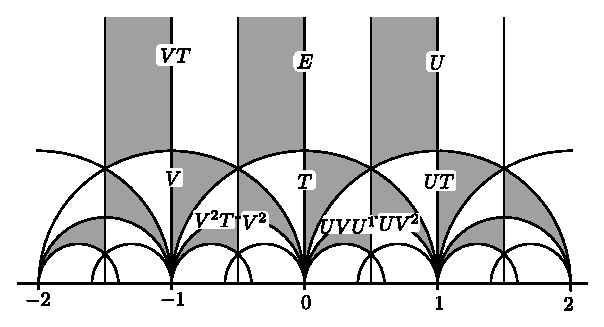
\includegraphics{vol29-fig/fig29-12.eps}
\smallskip
\caption{}
\label{chap2:fig12}
\end{figure}

\begin{thm}\label{chap2:thm8}
The \pageoriginale transformations $T = \left(\begin{smallmatrix}
0 &1\\-1& 0
\end{smallmatrix}\right)$ and $W=-V=-U^{-1}T=\left(\begin{smallmatrix}
-1 &-1\\1& 0
\end{smallmatrix}\right)$ generate the modular group $\Gamma$. They
satisfy the relations 
$$
T^4 = W^3 = E, \quad WT^2 = T^2W 
$$
and these are the defining relations for the group.
\end{thm}

\begin{proof}
Since $U$ and $T$ are the boundary substitutions of the normal
fundamental domain $\mathfrak{F}$ for $\Gamma$ given in \eqref{c2:eq1:1}, the
transformations $U$ and $T$ and therefore $W=-V=-U^{-1}T$ and $T$
generate $\Gamma$.
\end{proof}

It can be easily verified that the generators satisfy the given
relations. Let $R=E$ be an arbitrary relation in $\Gamma$. Without
loss of generality, we can assume that 
$$
R \equiv T^{v_1} W^{u_1} T^{v_2} W^{u_2} T^{v_2} \cdots W^{u_n}=E.
$$

With the help of the given relations and cyclic permutations of the
factors, we transform this relation into a reduced relation of the
type
$$
M_n = T^{e_1} W^{e_1} T^{e_2} W^{e_2} \cdots T^{e_n} W^{e_n} = T^{2e_0}
$$
with $e_0=0$ or 1 and $e_i=\pm 1 (i=1,2,\ldots, n)$. We shall show
that necessarily $n=0$ i.e. any given relation is a consequence of the
relations mentioned in the theorem, and this will complete the
proof. We prove, by induction on $n$, that if $M_n = \left(\begin{smallmatrix}
a_n &b_n\\c_n& d_n
\end{smallmatrix}\right)$, then $a_n, b_n, c_n, d_n \geq 0$ for $n\geq
1$ and moreover $b_n$ and $c_n$ are not simultaneously zero. When
$n=1$, 
$$
M_1 = \begin{pmatrix}
1&0\\1&1
\end{pmatrix} \text{ or } \begin{pmatrix}
1&1\\0&1
\end{pmatrix}
$$
according as $e_1=1$ or $-1$. Let us assume that the assertion is true
for $M_n$. \pageoriginale Then
\begin{align*}
M_{n+1} & = M_n T^{e_{n+1}} W^{e_{n+1}}\\
& = \begin{pmatrix}
a_n+b_n & b_n\\
c_n +d_n & d_n
\end{pmatrix} \text{ or } \begin{pmatrix}
a_n & a_n + b_n\\
c_n & c_n + d_n
\end{pmatrix}
\end{align*}
according as $e_{n+1}=1$ or $-1$. This shows that the relation $M_n=E$
is satisfied if and only if $n=0$ and consequently $e_0=0$.

Finally, we shall mention the use of the modular group in the
reduction theory of positive definite binary quadratic
forms. Throughout our discussion, we shall consider two-rowed real
position symmetric matrices as associated to positive definite binary
quadratic forms. Let
$A=\left(\begin{smallmatrix}a_0&a_1\\a_1&a_2 \end{smallmatrix}\right)$
be a real symmetric matrix. Then $A$ is positive $(A>0)$ if and only
if $a_0>0$ and $a_0a_2 - a^2_1>0$.

\begin{defi*}
Two positive symmetric matrices $A$ and $B$ are said to be
\textit{equivalent} if there exists an integral matrix $S$ with
$|S|=\pm 1$ such that $B=SAS'$ where $S'$ is the transpose of $S$. We
say that $A$ and $B$ are \textit{properly equivalent} if $|S|=1$. If
$A=\left(\begin{smallmatrix} a_0 & a_1\\ a_1
  &a_2\end{smallmatrix}\right)>0$, then the polynomial
$$
(1 \; \xi) A \begin{pmatrix}
1\\\xi  \end{pmatrix} = a_0 + 2 a_1 \xi + a_2 \xi^2
$$
has complex conjugate zeros. Let the two zeros be $-\tau$ and
$-\overline{\tau}$, such that $\tau$ belongs to $\mathscr{G}$. Then 
$$
a_0+2a_1\xi+a_2 \xi^2 = a_2 (\xi + \tau)(\xi+\overline{\tau}).
$$

We shall say that the point $\tau \in \mathscr{G}$ obtained in
this way is \textit{associated to the matrix} \pageoriginale
$A$. Obviously
$$
2a_1/a_2 = \tau + \overline{\tau} = 2x, a_0/a_2 = \tau \overline{\tau}
= x^2+y^2 (\tau =x+iy).
$$ 

If $w=\sqrt{|A|}>0$, then 
\begin{align*}
w^2 = a_0 a_2 - a^2_1 & = a^2_2 (a_0/a_2-a^2_1/a^2_2)\\
& = a^2_2 (x^2+y^2-x^2) = a^2_2 y^2.
\end{align*}

This shows that the matrix $A$ has the representation
$$
A = \frac{w}{y} \begin{pmatrix}
x^2+y^2 & x\\
x & 1
\end{pmatrix}.
$$

If $B = \left(\begin{smallmatrix} b_0 & b_1\\b_1 &
  b_2 \end{smallmatrix}\right)$ is another positive symmetric matrix
equivalent to $A$ i.e. $B=SAS'$, where $S$ is some integral matrix of
determinant $\pm 1$, then $|B|=|A|$ and therefore 
$$
B=\frac{w}{y^{\ast}} \begin{pmatrix} 
x^{\ast 2} + y^{\ast 2} & x^{\ast}\\
x^{\ast} & 1
\end{pmatrix}
$$
with some $\tau^{\ast} = x^{\ast} + iy^{\ast}$ such that
$-\tau^{\ast}$ and $-\overline{\tau}^{\ast}$ are the zeros of the
polynomial
$$
(1\xi) B \begin{pmatrix}
1\\\xi
\end{pmatrix} = b_0 + 2b_1 \xi + b_2 \xi^2.
$$

But with $\left(\begin{smallmatrix}
  a&b\\c&d \end{smallmatrix}\right)$, we have
\begin{align*}
(1 \; \xi) B \begin{pmatrix} 1\\\xi
  \end{pmatrix} & = (1 \; \xi) S A S' \begin{pmatrix}
1\\\xi
  \end{pmatrix}\\
& = (1 \; \xi) \begin{pmatrix}
a&b\\c&d
  \end{pmatrix} \begin{pmatrix}
a_0 &a_1 \\a_1 &a_2
  \end{pmatrix} \begin{pmatrix}
a&c\\b&d
  \end{pmatrix} \begin{pmatrix}
1\\\xi
  \end{pmatrix}\\
& = (a+c\xi b+\xi d) \begin{pmatrix}
a_0& a_1\\a_1& a_2
  \end{pmatrix} \begin{pmatrix}
a&+&c\xi\\
b &+& d\xi
  \end{pmatrix}\\
& = (a+c\xi)^2 a_0 + 2 a_1 (b+d\xi) (a+c\xi) + a_2 (b+d\xi)^2\\
& = a_2 \{(a+c\xi)^2 \tau \overline{\tau} + (\tau + \overline{\tau})
  (b+ d\xi) (a+c\xi) + (b+d\xi)^2\}\\
& = a_2 \{(a+c\xi) \tau + (b+d\xi)\} \{(a+c\xi)
  \overline{\tau}+(b+d\xi)\} \\
& = a_2 \{\xi (c\tau + d) + (a\tau + b)\} \{\xi (c\overline{\tau}+d) +
  a \overline{\tau}+b\}\\
& = a_2 |c\tau + d|^2 (\xi+S<\tau>) (\xi + S<\overline{\tau}>);
\end{align*}\pageoriginale
therefore 
\begin{align*}
\tau^{\ast} & = S <\tau> \text{ for } |S|=1.\\
\tau^{\ast} & = S (\overline{\tau}) \text{ for } |S|=-1.
\end{align*}

We shall say that a \textit{positive symmetric matrix $A$ is reduced}
when the point $\tau \in \mathscr{G}$ associated to $A$
belongs to the fundamental domain $\mathfrak{F}$, of the modular group
given in $(1)$. We have proved that in an equivalence class of properly
equivalent matrices there always exists a reduced matrix and this
matrix is uniquely determined if the associated point $\tau$ belongs
to the interior of $\mathfrak{F}$.
\end{defi*}

\section{Subgroups of the Modular Group}\label{chap2:sec2}

In general, here and in the following, we shall consider those
subgroups $\Gamma^{\ast}$ of $\Gamma$ which contain $-E$ and are of
finite index in $\Gamma$. We shall denote the index
$(\Gamma:\Gamma^{\ast})$ of $\Gamma^{\ast}$ in $\Gamma$ by $\mu$. Let
$S_1, S_2, \ldots, S_{\mu}$ be a complete system of representatives
of the right cosets of $\Gamma$ by $\Gamma^{\ast}$, so that 
$$
\Gamma = \bigcup^{\mu}_{i=1} \Gamma^{\ast} S_i.
$$

If \pageoriginale $\mathfrak{F}$ is a normal fundamental domain for
$\Gamma$, we shall show that $\mathfrak{F}^{\ast}$ given by 
$$
\mathfrak{F}^{\ast} = \bigcup^{\mu}_{i=1} \mathfrak{F}_{S_i}
$$
is a fundamental domain for $\gamma^{\ast}$. Since 
$$
\bigcup_{L\in \Gamma^{\ast}} \mathfrak{F}^{\ast}_L =
\bigcup_{L\in \Gamma^{\ast}} \bigcup^{\mu}_{i=1}
\mathfrak{F}_{LS_i} = \bigcup_{L \in \Gamma} \mathfrak{F}_L =
\mathscr{G}, 
$$
$\mathfrak{F}^{\ast}$ contains atleast one point from each set of
equivalent points with respect to $\Gamma^{\ast}$. In order to prove
that $\mathfrak{F}^{\ast}$ is a fundamental domain for
$\Gamma^{\ast}$, it remains to show that if $\tau$ belongs to
$\mathfrak{F}^{\ast} \cap \mathfrak{F}^{\ast}_L$ for some
$L\in \Gamma^{\ast}$, $L\neq \pm E$, then $\tau$ belongs to
the boundary of $\mathfrak{F}^{\ast}$. Our assumption $\tau\in
\mathfrak{F}^{\ast} \cap \mathfrak{F}^{\ast}_L$ for some $L$ in
$\Gamma^{\ast}$ implies that $\tau$ is in $\mathfrak{F}_{S_i} \cap
\mathfrak{F}_{LS_j}$ for some $i,j$ with $1\leq i, j\leq \mu$. If
$\mathfrak{F}_{LS_j} = \mathfrak{F}_{s_h}$ for some $h$ so that $LS_j
= \pm S_h$, we obtain $j=h$ and $L=\pm E$, contradicting our
assumption. Therefore $\mathfrak{F}_{LS_j} \neq \mathfrak{F}_{S_h}$
for $1\leq h \leq \mu$. Now it is obvious that the interior points of
$\mathfrak{F}_{LS_j}$ are exterior points of $\mathfrak{F}^{\ast}$;
consequently, $\tau$ is a boundary point of $\mathfrak{F}^{\ast}$ and
therefore of $\mathfrak{F}^{\ast}_L$. Hence $\mathfrak{F}^{\ast}$ is a
fundamental domain for the group $\Gamma^{\ast}$. Conversely, if the
set $\mathfrak{F}^{\ast} = \bigcup\limits^{t}_{i=1} \mathfrak{F}_{s_i}$,
where $S_i \in \Gamma$, is a fundamental domain for
$\Gamma^{\ast}$, then it can be easily proved that $t=\mu$ and $\{S_1,
S_2, \ldots, S_{\mu}\}$ is a complete set of coset representatives of
$\Gamma$ modulo $\Gamma^{\ast}$.

It is obvious that the parabolic cusps of $\Gamma^{\ast}$ are the same
as those of $\Gamma$, namely the rational points on the real axis and
$\infty$. Let $s_1,s_2, \ldots, s_{\sigma}$ \pageoriginale be a
complete system of inequivalent parabolic cusps of
$\Gamma^{\ast}$. There exist transformations $A_i$ in $\Gamma$ such
that 
$$
A^{-1}_i <\infty>  = s_i, i=1,2, \ldots , \sigma.
$$

Consider the group $A_i \Gamma^{\ast} A^{-1}_i$; it has $\infty$ as a
fixed point and therefore contains $U^r$ for some integer $r$. 
Let $N_i>0$ be so determined that $U^{N_i}$ is the least positive
power of $U$ belonging to the group $A_i \Gamma^{\ast} A^{-1}_i$. Then
the transformations $-E$ and $U^{N_i}$ generate the group contained in
$A_i \Gamma^{\ast}A^{-1}_i$ which leaves $\infty$ fixed. The integer $N_i$
determined above does not depend upon the choice of the cusp $s_i$ in
the class of $s_i$. If $s'_i=L<s_i>$ for $L \in
\Gamma^{\ast}$ and $B^{-1}_i <\infty> = s'_i$ for some $B_i
\in \Gamma$, then 
\begin{align*}
 &s_i = A^{-1}_{i}<\infty>   = L^{-1} B^{-1}_i <\infty>
  \Longrightarrow
  A_i L^{-1} B^{-1}_i <\infty>  = \infty \Longrightarrow\\
 \Longrightarrow \quad &  A_i L^{-1} B^{-1}_i  = \pm U^r \text{ for some
   integral } r \Longrightarrow\\
\Longrightarrow  \quad  &  A_i \Gamma^{\ast} A^{-1}_i  = U^r B_i \Gamma^{\ast}
B^{-1}_i U^{-r} \Longrightarrow U^{N_i} \in B_i \Gamma^{\ast} B^{-1}_i.
\end{align*}

This shows that if $U^{N'_i}$ is the least positive power of $U$
belonging to $B_i \Gamma^{\ast} B^{-1}_i$, then $N'_i \leq
N_i$. Similarly we get $N_i \leq N'_i$, which proves that $N'_i =
N_i$. We shall call the integer $N_i$ the \textit{width of the cusp
  sector} at the cusp $s_i$. We shall now construct a fundamental
domain for $\Gamma^{\ast}$ which shows a connection between $\mu$ and
the widths of cusp sectors at the various cusps of $\Gamma^{\ast}$. As
we have seen above, it is sufficient to give a coset decomposition of
$\Gamma$ modulo $\Gamma^{\ast}$ which indicates the desired
connection. We shall show that $\bigcup\limits^{\sigma}_{i=1}
\bigcup\limits^{N_i-1}_{r=0}\Gamma^{\ast} A^{-1}_i U^r$, where $A_i
\in \Gamma$ and $N_i >0$ as determined above, is a coset
decomposition of $\Gamma$ modulo $\Gamma^{\ast}$. If $S \in
\Gamma$, then, \pageoriginale for some $i$ with $1\leq i \leq \mu$ and
$L \in \Gamma^{\ast}$, we have 
$$
S <\infty> = L<s_i> = L A^{-1}_i <\infty> \Longrightarrow S = \pm L
A^{-1}_i U^t \text{ for some } t.
$$ 

Let $t=aN_i + r$ with $0\leq r < N_i$, then 
$$
S =\pm L (A^{-1}_i U^{N_i}A_i)^a A^{-1}_i U^r \in
\Gamma^{\ast}A^{-1}_i U^r. 
$$

Hence we obtain that 
\begin{equation*}
\Gamma = \bigcup^{\sigma}_{i=1} \bigcup^{N_i-1}_{r=0} \Gamma^{\ast}
A^{-1}_i U^r. \tag{1}\label{c2:eq2:1}
\end{equation*}

Moreover, if $S$ is a common element of $\Gamma^{\ast} A^{-1}_i U^r$
and $\Gamma^{\ast}A^{-1}_j U^s$ with $1\leq i, j\leq \sigma, 0\leq s <
N_j$ and $0\leq r<N_i$, then $S<\infty>$ is equivalent to both $s_i$
and $s_j$ with respect to $\Gamma^{\ast}$. Because of the choice of
the cusps, this is possible only if $i=j$, therefore $A^{-1}_i
U^{r-s}A_i$ belongs to $\Gamma^{\ast}$ showing that $r-s\equiv 0(\text{mod }
N_i)$. But $0\leq r, s< N_i$; therefore $s=r$ and this completely
proves that the decomposition of $\Gamma$ given in $(1)$ is a coset
decomposition of $\Gamma$ modulo $\Gamma^{\ast}$. Hence
\begin{equation*}
\mathfrak{F}^{\ast} =
\bigcup^{\sigma}_{i=1}\left(\bigcup^{N_i-1}_{r=0}
\mathfrak{F}_{U^r}\right)_{A^{-1}_i} \tag{2}\label{c2:eq2:2}
\end{equation*}
is a fundamental domain for $\Gamma^{\ast}$, which we shall use in the
sequel. If $\mathfrak{F}$ is the fundamental domain for $\Gamma$ given
by~\ref{c2:eq2:1} of the previous section, the $\left(\bigcup\limits^{N_i-1}_{r=0}
\mathfrak{F}_{U^r}\right)_{A^{-1}_i}$ is a cusp sector at the cusp
$s_i$ and the width of this sector is nothing but the ordinary width
of $\bigcup\limits^{N_i-1}_{r=0} \mathfrak{F}_{U^r}$, namely $N_i$. In
particular, we obtain that 
\begin{equation*}
(\Gamma:\Gamma^{\ast}) = \mu = N_1 
+ N_2 + \cdots + N_{\sigma}. \tag{3}\label{c2:eq2:3}
\end{equation*}

Obviously, \pageoriginale the elliptic fixed points of $\Gamma^{\ast}$
are either equivalent to $i$ or $\mathfrak{e}=e^{2\pi i/3}$ with
respect to $\Gamma$; therefore an elliptic fixed point of
$\Gamma^{\ast}$ is either of ramification index 1 or 2. Let $e_1$
(respectively $e_2$) denote the number of elliptic fixed points of
$\Gamma^{\ast}$ of ramification index 1 (respectively 2). Since
$\mathfrak{I}(\mathfrak{F}^{\ast})=\dfrac{\mu\pi}{3}$, we see from
formula~\eqref{c2:eq2:1} in chapter~\ref{chap1}, \S~\ref{chap1:sec4} 
that the genus $p$ of the Riemann
surface associated to the group $\Gamma^{\ast}$ is given by 
$$
p = \frac{\mu}{12} + 1 - \frac{\sigma}{2} - \frac{e_1}{4} - \frac{e_2}{3}.
$$

Let us further assume that $\Gamma^{\ast}$ is a normal subgroup of
$\Gamma$. If $\tau_1$ and $\tau_2$ are two points of $\mathscr{G}$
equivalent with respect to $\Gamma$, then the subgroups $\Gamma_1$ and
$\Gamma_2$ of $\Gamma^{\ast}$ which leave respectively $\tau_1$ and
$\tau_2$ fixed, are conjugate subgroups in $\Gamma$. Let
$\tau_2=A<\tau_1>$ with $A\in \Gamma$. Then the group $A^{-1}
\Gamma_2 A \subset A^{-1} \Gamma^{\ast} A = \Gamma^{\ast}$ leaves
$\tau_1$ fixed, therefore $A^{-1}\Gamma_2 A \subset
\Gamma_1$. Similarly $A\Gamma_1 A^{-1}\subset \Gamma_2$. Hence $A^{-1}
\Gamma_2 A = \Gamma_1$ and therefore the fixed points of
$\Gamma^{\ast}$ which are equivalent with respect to $\Gamma$ are of
the same type. In particular, all the widths of the cusp sectors at
various parabolic cusps of $\Gamma^{\ast}$ are equal and we obtain
from~\ref{c2:eq2:3}
$$
\mu = N \sigma, \text{ if } N_i = N \text{ for } i = 1, 2, \ldots, \sigma.
$$

Moreover, $e_1=N$ or $0$ (respectively $e_2=N$ or 0) according as $i$
(respectively $\rho$) is a fixed point of $\Gamma^{\ast}$ or
not. Thus we obtain the following table the genus of a normal
subgroup $\Gamma^{\ast}$ of $\Gamma$: 
\begin{center}
%\renewcommand{\arraystretch}{2}
%\tabcolsep=13pt
\begin{equation*}
\begin{array}{|c|c|}
    \hline
    p   & \mbox{ Fixed points of } \Gamma^{\ast}\\
    \hline
1 -\dfrac{\mu}{2}  \left(\dfrac{1}{N}+1\right) & i, \rho, \infty\\[5pt]
1 -\dfrac{\mu}{2}  \left(\dfrac{1}{N}+\dfrac{1}{2}\right) & \rho,
    \infty\\[5pt]
1 -\dfrac{\mu}{2}  \left(\dfrac{1}{N}+\dfrac{1}{3}\right) & i,
    \infty\\[5pt]
1 -\dfrac{\mu}{2}  \left(\dfrac{1}{N}-\dfrac{1}{6}\right) &
    \infty\\[5pt]
    \hline
\end{array}\tag{4}\label{c2:eq2:4}
\end{equation*}
\end{center}\pageoriginale 

In the above table, $\mu$ is the index of $\Gamma^{\ast}$ in $\Gamma$
and $N$ is the width of the cusp sector at any parabolic cusp of
$\Gamma^{\ast}$. 

Let $N$ be a natural number. Then the set of matrices $S\in
\Gamma$ with 
$$
S = \begin{pmatrix}
a&b\\c&b
\end{pmatrix} \equiv \begin{pmatrix}
1& 0\\
0 &1
\end{pmatrix} (\text{mod } N)
$$
form a group which we shall denote by $\Gamma[N]$. In the following,
we shall determine the index $\mu(N)$ of $\Gamma[N]$ in $\Gamma$. It
is obvious that two matrices $A$ and $B$ of $\Gamma$ belong to the
same coset of $\Gamma$ modulo $\Gamma[N]$ if and only if 
$$
A\Gamma[N] = B\Gamma[N] \Longleftrightarrow A^{-1} B \in
\Gamma[N] \Longleftrightarrow A\equiv B (\text{mod } N).
$$

This means that $\mu(N)$ is the number of matrices $S$ of $\Gamma$
which are incongruent modulo $N$. We assert that
$\mu(N)$ is also the number of integral matrices
$S=\left(\begin{smallmatrix} a&b\\c&d \end{smallmatrix}\right)$ which
are incongruent modulo $N$ and for which the determinant
$|S|=ad-bc\equiv 1(\text{mod  }N)$. In order to prove this assertion, 
\pageoriginale we have to show that for any matrix
$S=\left(\begin{smallmatrix}  a&b\\c&d\end{smallmatrix}\right)$ with
  $ab-bc \equiv 1(\text{mod } N)$, there exists a matrix $S_1$ in with
  $S_1\equiv S(\text{mod } N)$. Since $ad-bc \equiv 1(\text{mod } N)$,
  it follows that $(c,d,N)=1$. Let $(d, N)=q$; then $(c,q)=1$ and
  there exists an integer $s$ such that    
$$
s \equiv d/p (\text{mod } N/q) \text{ and } (s,c) = 1.
$$

This shows that $d'=sq=d+rN$ is such that $(d',c)=1$ and
$\left(\begin{smallmatrix} a&b\\c&d'  \end{smallmatrix}\right) \equiv
\left(\begin{smallmatrix}  a&b\\c&d\end{smallmatrix}\right) (\text{mod }
  N)$. Let $ad'-bc=1+wN$. Consider the matrix
  $\left(\begin{smallmatrix} a+xN & b+yN\\c &
    d' \end{smallmatrix}\right) $ where $x$ and $y$ are integers so
  determined that $xd'-yc=w$; such integers $x$
  and $y$ exist, because $(c,d')=1$. It is obvious that
  $\left(\begin{smallmatrix}a+xN&b+yN\\c&d' \end{smallmatrix}\right)$
  is a desired matrix $S_1\equiv S (\text{mod } N)$.

The function $\mu(N)$ is a multiplicative function of $N$ i.e. 
$$
\mu(N_1 \; N_2) = \mu (N_1) \mu (N_2) \text{ for } (N_1, N_2) = 1.
$$

For the proof, we observe that a solution $S=
\left(\begin{smallmatrix}  a&b\\c&d\end{smallmatrix}\right) $ of the
  matrix congruences 
$$
S\equiv S_i (\text{mod } N_i) \; (i=1,2)
$$
exists and is uniquely determined modulo $N_1N_2$, since
$(N_1,N_2)=1$. Further, $|S_i|\equiv 1(\text{mod } N_i)$ for $i=1,2$ imply
that $|S|\equiv 1 (\text{mod } N_1N_2)$ and vice versa. The assertion is now a
consequence of 
$$
S\text{mod } N_1 N_2 \leftrightarrow S_i\text{mod } N_i \; (i=1,2).
$$

Thus, in order to evaluate $\mu(N)$, it is sufficient to determine its
value of $N=p^{\alpha}$, where $p$ is a prime number.

Let $\mu_k(p^{\alpha})$, for $0\leq k \leq \alpha$, denote the number
of solutions of 
$$
ad - bc \equiv 1 (\text{mod } p^{\alpha}), (a, p^{\alpha}) = p^k,
$$\pageoriginale
which are distinct modulo $p^{\alpha}$.
\begin{enumerate}
\renewcommand{\labelenumi}{\theenumi)}
\item $\underline{k=0}$. The congruence $ad\equiv 1+bc(\text{mod }
  p^{\alpha})$ will have a unique solution for $d$ modulo
  $p^{\alpha}$ when $b$ and $c$ are given arbitrarily modulo
  $p^{\alpha}$. But a modulo $p^{\alpha}$ can be any one of the
  $\varphi(p^{\alpha})$ prime residue classes modulo $p^{\alpha}$;
  therefore $\mu_0(p^{\alpha})=p^{2\alpha}\varphi(p^{\alpha})$.

\item $\underline{k\geq 1}$. Let, first of all, a be fixed. Then the
  congruence 
$$
ad \equiv 1 + bc (\text{mod } p^{\alpha}), \; (a, p^{\alpha}) = p^k
$$
will have a solution for $d$, if and only if $l+bc\equiv 0(\text{mod }
p^k)$. For a given $b$, the congruence $bc\equiv -1(\text{mod } p^k)$ will
have a unique solution for $c\text{mod } p^k$ and therefore $p^{\alpha-k}$
solutions modulo $p^{\alpha}$. But, for $b$, we can take any of the
$\varphi(p^{\alpha})$ prime residue classes modulo $p^{\alpha}$;
therefore, the number of solutions modulo $p^{\alpha}$ of $bc\equiv
-1(\text{mod } p^k)$ is $p^{\alpha -k}\varphi(p^{\alpha})$. For fixed $a,b$
and $c$, the congruence $ad\equiv 1+bc (\text{mod } p^{\alpha})$ determines
$d$ uniquely modulo $p^{\alpha -k}$. This means that, for fixed $a$,
$b$ and $c$, the congruence $ad\equiv 1 + bc (\text{mod } p^{\alpha})$ has
$p^k$ solutions $d$ modulo $p^{\alpha}$ and therefore, for fixed a,
it has $\varphi(p^{\alpha}) \; p^{\alpha}$ solutions. Since, for a fixed
$k$, the integer a with $(a,p^{\alpha})=p^k$ has
$\varphi(p^{(\alpha-k)})$ distinct values modulo $p^{\alpha}$, we see
that 
$$
\mu_k(p^{\alpha}) = \varphi(p^{\alpha - k}) \varphi(p^{\alpha}) p^{\alpha}
\text{ for } k \geq 1.
$$
\end{enumerate}

The cases 1) and 2) above together give 
\begin{align*}
\mu(p^{\alpha}) & = \mu_0(p^{\alpha}) + \sum^{\alpha}_{k=1} \mu_k
(p^{\alpha})\\
&= \phi (p^{\alpha}) p^{2\alpha}+ \sum^{\alpha}_{k=1}
\varphi(p^{\alpha-k}) \varphi(p^{\alpha}) p^{\alpha}\\
& = p^{\alpha}\; \varphi \; (p^{\alpha}) \{p^{\alpha}+
(p^{\alpha-1}-p^{\alpha-2}) + (p^{\alpha -2} - p^{\alpha-3})\\ 
&\qquad{}+ \cdots + p-1+1\}\\
& = p^{3\alpha}(1-p^{-2}).
\end{align*}\pageoriginale

Hence we obtain that 
\begin{equation*}
\mu(N) = N^3 \prod_{p|N} (1-p^{-2})
 (p \text{ a prime number } >0). \tag{5}\label{c2:eq2:5}
\end{equation*}

Obviously, the group $\Gamma[N]$ does not contain $-E$ for $N>2$. Let
$\Gamma^{\ast}[N]$ denote the group generated by $-E$ and $\Gamma[N]$,
so that 
$$
\Gamma^{\ast} [N] = \{S|S \in \Gamma, S \equiv \pm E (\text{mod } N)\}.
$$

The index $\mu^{\ast} (N) = (\Gamma : \Gamma^{\ast}[N])$ is given by 
\begin{equation*}
\mu^{\ast} (N) = \begin{cases}
\mu(N) = 6, & \text{for } N=2\\
\frac{1}{2} \mu(N) = \frac{1}{2} N^3 & \prod_{p|N} (1-p^{-2}), \text{
  for } N >2.
\end{cases} \tag{6}\label{c2:eq2:6}
\end{equation*}

We call $\Gamma^{\ast}[N]$ \textit{the principal congruence subgroup of
  level} $N$. It is a normal subgroup of
  $\Gamma$. Obviously, $N$ is the width of the cusp sector at any
  parabolic cusp of $\Gamma^{\ast}[N]$ and therefore
  $\mu^{\ast}(N)/N$ is the number of inequivalent parabolic cusps of
  $\Gamma^{\ast}[N]$. Since, for $N>1$, $\Gamma^{\ast}[N]$ contains
  neither $T=\left(\begin{smallmatrix}
    0&1\\-1&0\end{smallmatrix}\right)n$ or $V =
    \left(\begin{smallmatrix} 1&1\\-1&0 \end{smallmatrix}\right)$,
    $i$ and $\rho$ are not fixed points of
    $\Gamma^{\ast}[N]$. Together with~\eqref{c2:eq2:4}, this shows that the genus
    $p(N)$, of $\Gamma^{\ast}[N]$, is given by 
$$
p(N)=1 + \frac{\mu^{\ast}(N)}{2} \left(\frac{1}{6} - \frac{1}{N}\right)
$$

Finally, we obtain by~\eqref{c2:eq2:5},
\begin{equation*}
p(N) = 
\begin{cases}
0, \quad \text{ for } N = 1, 2, 3, 4, 5.\\
1 + \frac{N^2(N-6)}{24} \prod\limits_{q|N} (1-q^{-2}), 
\end{cases}\tag{7}\label{c2:eq2:7}
\end{equation*}\pageoriginale
where $q$ runs over positive prime divisors of $N$. 

A subgroup $\Gamma^{\ast}$ of $\Gamma$ is called a \textit{congruence
  subgroup}, if $\Gamma^{\ast}$ contains a principal congruence
subgroup of level $N$ for some $N \geq 1$. The following remarkable
theorem of Fricke-Wohlfahrt enables us to associate with
$\Gamma^{\ast}$ a uniquely determined principal congruence subgroup.

\begin{thm}\label{chap2:thm9}
Let $N_1, N_2, \ldots , N_{\sigma}$ be the widths of the cusp sectors
of a complete system of inequivalent parabolic cusps of a congruence
subgroup $\Gamma^{\ast}$ and $\overline{N}$ the least common multiple
of $N_1, N_2, \ldots,N_{\sigma}$. Then $\Gamma^{\ast}[N] \subset
\Gamma^{\ast}$ if and only if $\overline{N}$ divides $N$.
\end{thm}

\begin{proof}
Let us assume that $\Gamma^{\ast}[N] \subset \Gamma^{\ast}$. Let $s_1,
s_2, \ldots , s_{\sigma}$ be a complete system of inequivalent
parabolic cusps of $\Gamma^{\ast}$  and let $A^{-1}_i<\infty> = s_i$,
$A_i \in \Gamma$ for $i = 1,2, \ldots, \sigma$. Then $N_i$ is
the least natural number with the property that $U^{N_i}$ belongs to
$A_i \Gamma^{\ast} A^{-1}_i$. But $\Gamma^{\ast} [N] \subset
\Gamma^{\ast}$; therefore 
$$
U^N \in \Gamma^{\ast} [N] = A_i \Gamma^{\ast} [N] A^{-1}_i
\subset A_i \Gamma^{\ast} A^{-1}_i.
$$

This implies that $N_i$ divides $N$ for $i=1,2,\ldots, \sigma$ and
therefore $\overline{N}$ divides $N$.
\end{proof}

Let $N$ be a natural number divisible by $\overline{N}$. In order to
prove that $\Gamma^{\ast}[N] \subset \Gamma^{\ast}$, it is sufficient
to prove that $\Gamma[\overline{N}] \subset \Gamma^{\ast}$, since
$-E\in \Gamma^{\ast}$ and $\Gamma^{\ast}[N]\subset
\Gamma^{\ast}[\overline{N}]$. Let $S =
\left(\begin{smallmatrix} a&b\\c&d \end{smallmatrix}\right)$ be an
arbitrary element of $\Gamma[\overline{N}]$.
\begin{enumerate}
\renewcommand{\theenumi}{\roman{enumi}}
\renewcommand{\labelenumi}{\theenumi)}
\item For \pageoriginale any matrix $A$ in $\Gamma$ and any integer
  $g$, we claim that 
$$
S_1 = A^{-1} \left(\begin{smallmatrix} 1&g\overline{N}\\ 0 &
  1 \end{smallmatrix}\right) \; A \in \Gamma^{\ast}.
$$

In fact, since $A^{-1} <\infty>$ is equivalent to $s_j$ with respect
to $\Gamma^{\ast}$ for some $j$ with $l\leq j \leq \sigma$ and since
$N_j$ divides $\overline{N}$, we see that
$\left(\begin{smallmatrix} 1 & g
  \overline{N}\\0&1 \end{smallmatrix}\right)\in A\Gamma^{\ast}
A^{-1}$, which implies our claim.

\item By the definition of $\Gamma^{\ast}$, there exists a natural
  number $n$ such that $\Gamma^{\ast}[n] \subset \Gamma^{\ast}$. Since
  $(c,d)=1$ and further $\overline{N}$ divides $d$, we have $(c
  \overline{N},d)=1$. Therefore, we can find an integer $g$ such that
  $d'=d+gc\overline{N}$ is coprime to $n$. But
  $\left(\begin{smallmatrix} 1 &g\overline{N}\\0 &
    1 \end{smallmatrix}\right) \in \Gamma^{\ast}$ in view of
  (i) with $A=E$. It follows that $S_2=S
  \left(\begin{smallmatrix}1&g\overline{N}\\ 0 &
    1\end{smallmatrix}\right)=
    \left(\begin{smallmatrix} a &
      ag\overline{N}+b\\c&d' \end{smallmatrix}\right)
    \in\Gamma^{\ast} \Longleftrightarrow S \in
    \Gamma^{\ast}$. Hence we may assume, in the sequel, that $(d,n)=1$ already.
 
\item Consider the matrix
$$
S_3 = \left(\begin{smallmatrix} a_3 &
  b_3\\c_3&d_3 \end{smallmatrix}\right)
= \left(\begin{smallmatrix} 1 & h\overline{N}\\ 0 &
  1 \end{smallmatrix}\right) S
\left(\begin{smallmatrix} 1&0\\g\overline{N}&
  1 \end{smallmatrix}\right) =
\left(\begin{smallmatrix}  \ast & b+dh\overline{N}\\ c+ d
  g\overline{N} & d \end{smallmatrix}\right)  
$$
where $g$ and $h$ are arbitrary integers. Since $S \in \Gamma[N]$,
we have $b=b_1 \overline{N}, c=c_1\overline{N}$ with integral $b_1,
c_1$. Now there exist integers $g,h$ such that $n$ divides both
$c_1+dg$ and $b_1+dh$. Thus $n$ divides both $b_3$ and $c_3$;
moreover, $d_3=d$ and so $(d_3,n)=1$, by (ii). Applying (i) with $A =
\left(\begin{smallmatrix} 0&1\\-1&0 \end{smallmatrix}\right)$, if
follows that $\left(\begin{smallmatrix} 1&0\\-g\overline{N}&
  1 \end{smallmatrix}\right)$ and therefore also
$\left(\begin{smallmatrix} 1&0\\g\overline{N}
  &1 \end{smallmatrix}\right)$ is in $\Gamma^{\ast}$. For the matrix
$S$, we could have thus assumed already, as in (ii) and we \textit{do}
indeed \textit{assume} in the sequel that $b\equiv c \equiv 0(\text{mod } n)$
and $(d,n)=1$. 
\end{enumerate}

We now \pageoriginale complete the proof of theorem~\ref{chap2:thm9}, using steps
(i)-(iii) above. Applying (i) with $A =
\left(\begin{smallmatrix} 1&0\\1&1 \end{smallmatrix}\right)$ shows
that $\left(\begin{smallmatrix} 1+g\overline{N} &
  g\overline{N}\\ -g\overline{N} & 1-g\overline{N}
\end{smallmatrix} \right)\in
  \Gamma^{\ast}$ for any integer $g$. Since $S \in
  \Gamma[\overline{N}]$, we have $a\equiv 1(\text{mod } \overline{N})$
  i.e. $a=1+g\overline{N}$ for an integer $g$. It follows that
  $\left(\begin{smallmatrix} a& a-1\\
1-a& 2-a \end{smallmatrix}\right) \in
  \Gamma^{\ast}$. Moreover, $d\equiv 1(\text{mod } \overline{N})$ and hence
  all the three matrices on the right hand side of
$$
\left(\begin{smallmatrix} a & ad-1\\
1-ad & d (2-ad)\end{smallmatrix}\right) = S_4 =
\left(\begin{smallmatrix} 1 & 0\\1-d & 1 \end{smallmatrix}\right)
\left(\begin{smallmatrix} a&a-1\\1-a& 2-a \end{smallmatrix}\right)    
\left(\begin{smallmatrix} 1 & d-1\\ 0&1 \end{smallmatrix}\right)
$$
are in $\Gamma^{\ast}$, implying that $S_4 \in
\Gamma^{\ast}$. Now
$$
SS^{-1}_4 = \left(\begin{smallmatrix}
  a&b\\c&d \end{smallmatrix}\right) 
\left(\begin{smallmatrix} d(2-ad) & 1-ad\\
ad-1 & a \end{smallmatrix}\right)\equiv
\left(\begin{smallmatrix} a&0\\0&d \end{smallmatrix}\right)
\left(\begin{smallmatrix}d&0\\0&a \end{smallmatrix}\right)\equiv E
(\text{mod } n),
$$
since $b\equiv c \equiv 0(\text{mod } n)$ and consequently $ad\equiv 1(\text{mod }
n)$. Thus $SS^{-1}_4 \in \Gamma^{\ast}[n] \subset
\Gamma^{\ast}$ which together with $S_4 \in \Gamma^{\ast}$
implies that $S \in \Gamma^{\ast}$, proving the theorem.

This theorem shows $\Gamma^{\ast}[\overline{N}]$ with $\overline{N}$
as defined above is the maximal principal congruence subgroup
contained in $\Gamma^{\ast}$. We shall call this uniquely determined
number $\overline{N}$ as \textit{the level of the congruence subgroup}
$\Gamma^{\ast}$. With the help of the above theorem, we shall show
later that there are subgroups of finite index in $\Gamma$ which are
\textit{not} congruence subgroups.

In what follows, unless otherwise stated, $\mathfrak{F}$ will denote
the normal fundamental domain of $\Gamma$ given by (1) of the previous
section. The congruence \pageoriginale subgroups $\Gamma_0[N]$ and
$\Gamma^0[N]$ ($N$ a natural number) defined by 
\begin{align*}
\Gamma_0 [N] & = \{S|S =
\left(\begin{smallmatrix}a&b\\c&d \end{smallmatrix}\right)\in\Gamma,
c\equiv 0 (\text{mod } N)\}\\
\Gamma^0 [N] & = T \Gamma_0 [N] T^{-1}
\end{align*}
are of some importance. Obviously $\Gamma_0[N]$ contains $\Gamma[N]$
and therefore
$$
(\Gamma:\Gamma_0[N]) = (\Gamma:\Gamma[N])/(\Gamma_0[N]:\Gamma[N]).
$$

But the index of $\Gamma[N]$ in $\Gamma_0[N]$ is equal to the number
of integral quadruples $a,b,c$ and $d$ incongruent modulo $N$ with
$ad\equiv 1(\text{mod } N)$ and $c\equiv 0(\text{mod } N)$; therefore
$(\Gamma_0N:\Gamma[N]) = N \varphi(N)$. Using~\eqref{c2:eq2:5}, we obtain
$$
(\Gamma:\Gamma_0 [N]) = \frac{\mu(N)}{N\varphi(N)} = N \prod_{q|N}
\left(1+\frac{1}{q}\right),
$$
where $q$ runs over positive prime divisors of $N$. It is obvious that
the group $\Gamma^0[N]$ defined above consists of the matrices $S=
\left(\begin{smallmatrix} a&b\\c&d \end{smallmatrix}\right)\in
\Gamma$ with $b\equiv 0(\text{mod } N)$ and further, $(\Gamma: \Gamma^0
      [N])=(\Gamma: \Gamma_0[N])$. Since 
$$
U^r \in \Gamma_0 [N] \Leftrightarrow r \equiv 0(\text{mod } 1), U^r
\in \Gamma^0 [N] \Leftrightarrow r \equiv 0(\text{mod } N), 
$$
the width of the cusp sector at the inequivalent cusps $\infty$ and 0
for $\Gamma_0[N]$ is 1 and N respectively and for $\Gamma^0[N]$ the
respective widths are $N$ and 1. If $N=q$ is a prime number, then
$$
\mathfrak{F}^{\ast} = \left\{ \bigcup^{q-l}_{j=0}
\mathfrak{F}_{U^j}\right\} \bigcup \mathfrak{F}_T,
$$
which consists of the two cusp sectors at the inequivalent cusps
$\infty$ and 0 for $\Gamma^0[q]$, is a fundamental domain of
$\Gamma^0[q]$. This is a consequence of relations (2) and (3), since
there are only two inequivalent parabolic cusps \pageoriginale for
$\Gamma^0[q]$.

We now consider some special subgroups of $\Gamma$. Let $K$ be the
commutator subgroup of $\Gamma$. In order to prove $(\Gamma:K)=12$, we
represent an arbitrary element $S$ in $\Gamma$ as $S=W^{a_1} T^{b_1}
W^{a_2} T^{b_2} \cdots W^{a_r} T^{b_r}$. According to the defining
relations for the generators $W$, $T$ of $\Gamma$ given in theorem~\ref{chap2:thm8},
the sums $e_1(S)=a_1+a_2+\cdots + a_r$ (respectively
$e_2(S)=b_1+b_2+\cdots + b_r$) are uniquely determined modulo 3
(respectively modulo 4). If $S$ is a commutator, it is obvious that
$e_1(S)\equiv 0(\text{mod } 3)$ and $e_2(S)\equiv 0(\text{mod } 4)$. Thus this is
true also for an arbitrary element of $K$, since $K$ is generated by
commutators. Since $e_1(W)\equiv 1(\text{mod } 3)$ and $e_2(T^2)\equiv 2(\text{mod }
4)$, it follows that $W$ and $T^2$ are not in $K$ but we have 
$$
(TK)^4 = (WK)^3 = K \text{ and } WTK = TWK.
$$

This proves that $\Gamma/K$ is an abelian group of order 12 and the
group $K^{\ast}$ generated by $K$ and $T^2(=-E)$ is a normal subgroup
of index 6 in $\Gamma$. Since $UK=T^3 W^{-1}K$ is an element of order
12 in $\Gamma/K$, we get $\Gamma=\bigcup\limits^5_{r=0}
K^{\ast}U^r$. This proves that $\mathfrak{F}^{\ast} =
\bigcup\limits^5_{r=0} \mathfrak{F}_{U^r}$ (see figure~\ref{chap2:fig13} is a
fundamental domain for $K^{\ast}$. Since the normal subgroup
$K^{\ast}$ does not contain both $T$ and $V$, neither $i$ nor $\rho$
is a fixed point of $K^{\ast}$. The width of the cusp sector at the
parabolic cusp of $\mathfrak{F}^{\ast}$ is 6; therefore, from~\eqref{c2:eq2:4},
we see that the genus of $K^{\ast}$ is 1. Since $T U^{-3} \equiv V^3
T^{-2}\equiv E(\text{mod } K^{\ast})$, it is obvious that the transformations
$$
A_1 = U^6, A_2 = TU^{-3}, A_3 = U T U^{-4}, A_4 = U^2 TU^{-5}
$$
belong to $K^{\ast}$. They are the boundary substitutions of
$\mathfrak{F}^{\ast}$; therefore together \pageoriginale with $-E$
they generate $K^{\ast}$.

\begin{figure}[H]
\centering
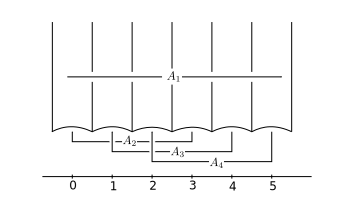
\includegraphics{vol29-fig/fig29-13.eps}
\smallskip
\caption{}
\label{chap2:fig13}
\end{figure}

We shall now show that the group $K^{\ast}$ is a congruence subgroup
of level 6. Let $\Gamma_0$ denote the group generated by
$\Gamma^{\ast}[6]$ and $K^{\ast}$. It can be verified that
$\Gamma_0/\Gamma^{\ast} [6]$ is an abelian group and moreover,
\begin{align*}
A^2_3 & \equiv A^4_2 (\text{mod } \Gamma^{\ast} [6])\\
A^5_2 A_3 & \equiv A_4 (\text{mod } \Gamma^{\ast} [6])\\
A_1 \equiv A^6_2 & \equiv E (\text{mod } \Gamma^{\ast}[6]). 
\end{align*}
showing \pageoriginale that, for $0\leq k < 6$ and $0\leq \ell < 2$,
$A^k_2 A^{\ell}_3 $ represent the cosets of $\Gamma_0$ modulo
$\Gamma^{\ast}[6]$. Thus
$(\Gamma_0:\Gamma^{\ast}[6])\leq 12$ and 
therefore
$$
6=(\Gamma:K^{\ast}) \geq (\Gamma:\Gamma_0) =
\frac{(\Gamma:\Gamma^{\ast} [6])}{(\Gamma_0:\Gamma^{\ast}[6])} \geq
\frac{72}{12} = 6, 
$$
which proves that $(\Gamma:K^{\ast})=(\Gamma:\Gamma_0)$ or $\Gamma_0 =
K^{\ast}$ and $\Gamma^{\ast}[6] \subset K^{\ast}$. The commutator
subgroup is a particular example of the so-called `cycloid subgroup'
of $\Gamma$. In general, a subgroup $Z$ of $\Gamma$ is said to be a
\textit{cycloid subgroup}, if the fundamental domain of $Z$ has only
one cusp sector i.e. $\sigma = 1$. If $\mu$ is the index of $Z$ in
$\Gamma$, then $\bigcup^{\mu-1}_{i=0} \mathfrak{F}_{U^i}$ is a
fundamental domain for $Z$ clearly. Petersson has constructed an
infinite number of cycloid subgroups of $\Gamma$ and proved that
exactly 1667868 are congruence subgroups thus showing that there are
infinitely many subgroups of $\Gamma$ which are not congruence
subgroups. He has further proved that all subgroups of index $\leq$ 6
in $\Gamma$ are congruence subgroups.

%%thm9
In the following, we shall determine all congruence subgroups of
$\Gamma$ of level 2. Let $\Gamma^{\ast}$ denote such a subgroup. Then,
by theorem~\ref{chap2:thm9}, $\Gamma^{\ast}$ contains $\Gamma^{\ast}[2] =
\Gamma[2]$. Since the index of $\Gamma[2]$ in $\Gamma$
is 6, the index 
of $\Gamma^{\ast}$ in $\Gamma$ is either 6 or 3 or 2. This shows that
$(\Gamma^{\ast} :\Gamma[2])=1,2,3$ according as
$(\Gamma:\Gamma^{\ast})=6,3,2$. 

Let $(\Gamma^{\ast}:\Gamma[2])=1$
i.e. $\Gamma^{\ast}=\Gamma[2]$. Since $U^2$ belongs to
$\Gamma[2]$, 
the width of the cusp sector at the cusp $\infty$ is 2. But
$\Gamma[2]$ is a normal subgroup of $\Gamma$ and therefore the width
of the cusp sector at any cusp of $\Gamma[2]$ is 2 and there are
three inequivalent cusps of $\Gamma[2]$, for example 0,1 and
$\infty$. It is obvious that 
$$
\mathfrak{F}^{\ast} = (\mathfrak{F}\cup \mathfrak{F}_U) \cup
(\mathfrak{F}_T \cup \mathfrak{F}_{TU}) \cup (\mathfrak{F}_{UT} \cup
\mathfrak{F}_{UTU}) 
$$\pageoriginale
is a fundamental domain for $\Gamma[2]$, because it consists of three
cusp sectors at the inequivalent cusps of $\Gamma[2]$.

\begin{figure}[H]
\centering
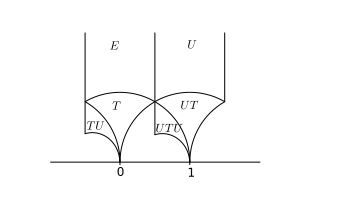
\includegraphics{vol29-fig/fig29-14.eps}
\smallskip
\caption{}
\label{chap2:fig14}
\end{figure}

It now follows that
$$
\Gamma = \Gamma [2] \cup \Gamma [2] U \cup \Gamma [2] T \cup \Gamma
       [2] TU \cup \Gamma [2] U T \cup \Gamma [2] U T U.
$$

If we replace some parts of $\mathfrak{F}^{\ast}$ in figure~\ref{chap2:fig14} by
suitable equivalent parts, then we obtain a fundamental domain as
shown in figure~\ref{chap2:fig15}.
\begin{figure}[H]
\centering
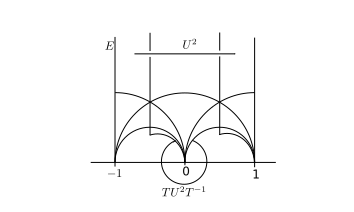
\includegraphics{vol29-fig/fig29-15.eps}
\smallskip
\caption{}
\label{chap2:fig15}
\end{figure}\pageoriginale

It is obvious that $U^2$ and $TU^2T^{-1}$ are in $\Gamma [2]$;
they are the boundary substitutions of the fundamental domain in
figure~\ref{chap2:fig15}. Therefore $U^2$ and $TU^2T^{-1}$ together with $-E$
generate $\Gamma[2]$.

Let $(\Gamma^{\ast}:\Gamma[2])=3$. Then
$\Gamma^{\ast}/\Gamma[2]$ is a Sylow subgroup of order 3 in
$\Gamma/\Gamma[2]$. But $\Gamma^{\ast}/\Gamma [2]$ is of
index 2 in $\Gamma/\Gamma[2]$; therefore it is a normal
subgroup. Hence $\Gamma^{\ast}/\Gamma[2]$ is uniquely determined
and therefore $\Gamma^{\ast}$ is a uniquely determined normal subgroup
of $\Gamma$. We shall denote it by $N_2$. The group $N_2/\Gamma
[2]$ is generated by any element of order 3. Since $V$ does not
belong to $\Gamma[2]$ and $V^3$ belongs to $\Gamma[2]$, we
have 
$$
N_2 = \Gamma[2] \cup \Gamma[2] V \cup \Gamma [2] V^2.
$$

Moreover $U$ does not belong to $N_2$; because, if $U$ belongs to
$N_2$, then $T=UV$ \pageoriginale belongs to $N_2$ implying that
$\Gamma=N_2$, a contradiction to $(\Gamma:N_2)=2$. Therefore 
$$
\Gamma = N_2 \bigcup N_2 U. 
$$
and $\mathfrak{F}^{\ast}=\mathfrak{F}\bigcup \mathfrak{F}_U$ (see
figure~\ref{chap2:fig16} is a fundamental domain for $N_2$ with the 
boundary substitutions $U^2$ and $U V U^{-1}$.
\begin{figure}[H]
\centering
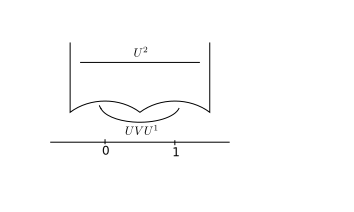
\includegraphics{vol29-fig/fig29-16.eps}
\smallskip
\caption{}
\label{chap2:fig16}
\end{figure}

Let $(\Gamma^{\ast}:\Gamma[2])=2$. Then
$\Gamma^{\ast}/\Gamma[2]$ is a Sylow subgroup of order 2 and
there are three conjugate Sylow subgroups of order 2 in $\Gamma/\Gamma
[2]$. One of these subgroups is the so-called \textit{theta-group}
$$
\Gamma_{\vartheta} = \Gamma [2] \bigcup \Gamma[2]T.
$$

The group $\Gamma_{\vartheta}$ consists of the matrices
$S=\left(\begin{smallmatrix}a&b\\c&d \end{smallmatrix}\right)$ in
$\Gamma$ with either $b\equiv c \equiv 0(\text{mod } 2)$ \pageoriginale or
$a\equiv d \equiv 0(\text{mod } 2)$ and it is not a normal subgroup of
$\Gamma$. The width of the cusp sector at $\infty$ is 2, because $U^2$
is the least positive power of $U$ belonging to
$\Gamma_{\vartheta}$. Since $(\Gamma:\Gamma_{\vartheta})=3$, we obtain
from~\eqref{c2:eq2:3} that $\Gamma_{\vartheta}$ has only one cusp, say 1
(inequivalent to $\infty$), the width of the cusp sector at which is
1. It is obvious that 
$$
\mathfrak{F}^{\ast} =(\mathfrak{F} \bigcup \mathfrak{F}_U) \bigcup
\mathfrak{F}_{UT} 
$$
is a fundamental domain for $\Gamma_{\vartheta}$, since it consists of
cusp sectors at the two inequivalent cusps of
$\Gamma_{\vartheta}$. Therefore $\Gamma=\Gamma_{\vartheta}\bigcup
\Gamma_{\vartheta} U \bigcup \Gamma_{\vartheta} UT$ is a coset
decomposition of $\Gamma$ modulo $\Gamma_{\vartheta}$. If we replace a
part of the above mentioned fundamental domain by a suitable equivalent
part, we obtain a fundamental domain $\mathfrak{F}^{\ast}$ given by 
$$
\mathfrak{F}^{\ast} = \{\tau |\tau = x+ iy, |x| \leq 1, |\tau| \geq
1\} \qquad (\text{see figure~\ref{chap2:fig17}})
$$
with the boundary substitutions $T$ and $U^2$.

\begin{figure}[H]
\centering
\includegraphics{vol29-fig/fig29-17.eps}
\smallskip
\caption{}
\label{chap2:fig17}
\end{figure}

The \pageoriginale above discussion shows that there exist only 5
congruence subgroups of $\Gamma$ of level 2. 

We shall now construct infinitely many subgroup of finite index in
$\Gamma$, which are not congruence subgroups. We consider
configurations I and II as shown in figure~\ref{chap2:fig18} and which formed by
images of $\mathfrak{F}$ or images of parts of $\mathfrak{F}$ under
$\Gamma$.

\begin{figure}[H]
\centering
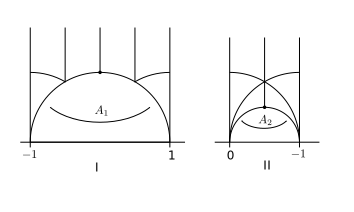
\includegraphics{vol29-fig/fig29-18.eps}
\smallskip
\caption{}
\label{chap2:fig18}
\end{figure}

We take a copies of the configuration $I$ and $b$ copies of the
configuration II and arrange them in some order so that the resulting
figure is a connected domain say $\mathfrak{F}^{\ast}$ (see figure~\ref{chap2:fig19}
for $a=3$, $b=2$), which has $i$ as a boundary point.

\begin{figure}[H]
\centering
\includegraphics{vol29-fig/fig29-19.eps}
\smallskip
\caption{}
\label{chap2:fig19}
\end{figure}\pageoriginale 

The transformations $A_1, A_2, \ldots, A_r(r=a+b)$ are elliptic
transformations of order 2, because they are conjugates of $T$ in
$\Gamma$. Any circular arc of the boundary of $\mathfrak{F}^{\ast}$ is
mapped onto itself by one of these elliptic transformations. The
vertical edges of $\mathfrak{F}^{\ast}$ are equivalent under
$P=U^{2a+b}$. Let $\Gamma^{\ast}$ denote the subgroup of $\Gamma$
generated by $P,A_1, \ldots, A_r$. We shall show that
$\mathfrak{F}^{\ast}$ is a fundamental domain for $\Gamma^{\ast}$ and
that for a suitable choice of $a$ and $b$, $\Gamma^{\ast}$ is not a
congruence subgroup. From the fact that $\mathfrak{F}^{\ast}$ is a
fundamental domain for $\Gamma^{\ast}$ (to be proved later), it is
obvious that $\Gamma^{\ast}$ has only two inequivalent parabolic
cusps, for example $\infty$ and 1, and the elliptic fixed points of
$\Gamma^{\ast}$ are equivalent to $i$ under $\Gamma$. Moreover, the
widths of the cusp sectors at $\infty$ and 1 are given by
$N_{\infty}=2a+b$, $N_1=a+2b$ respectively. Using (3), we get $\mu =
(\Gamma:\Gamma^{\ast}) = N_{\infty}+N_1=3(a+b)$. Let us suppose that
$\Gamma^{\ast}$ is a congruence subgroup of level $N$. Let us assume
that $p=a+b$ is a prime number and $a,b\geq 2$. Since $\Gamma\supset
\Gamma^{\ast} \supset \Gamma [N]$, $\mu$ divides $\mu(N)$ and
therefore $p$ divides 
$$
\mu(N) = N^3 \prod_{q|N} (1-q^{-2}) = N^{\ast} \prod_{q|N} (q^2-1)
(N|N^{\ast}|N^3, q \text{ a prime number}).
$$\pageoriginale 

But $N$, by theorem~\ref{chap2:thm9}, is the least common multiple of
$N_{\infty}=p+a$ and $N_1 = p + b$, therefore $p$ does not divide
$N$. Thus $p$ divides $(q^2-1)$ for at least one prime $q$ dividing
$N$. Since $p\geq 5$, $q\pm 1$ is even and $p$ divides
$\dfrac{1}{2}(q\pm 1)$. Obviously, $q$ divides either $p+a$ or $p+b$,
because $q$ divides $N$ which is the least common multiple of $p+a$
and $p+b$. But $a, b\geq 2$ and $a+b=p$, therefore $q\leq 2 p-2$. This
shows that $p$ divides $\dfrac{1}{2}(q\pm 1)$ which is different from
zero and strictly less than $p$. Hence our supposition that
$\Gamma^{\ast}$ is a congruence subgroup is false when $a+b=p$ is a
prime number and $a,b\geq 2$. But there are infinitely many pairs of
natural numbers $(a,b)$ with the above property; therefore our
assertion that there exist infinitely many subgroups of $\Gamma$ of
finite index which are not congruence subgroups is proved.

We shall prove now that $\mathfrak{F}^{\ast}$ is a fundamental domain
for $\Gamma^{\ast}$. In order to prove that $\mathfrak{F}^{\ast}$
contains atleast one point from each set of equivalent points under
$\Gamma^{\ast}$, it is sufficient to prove that $\mathscr{G} =
\bigcup_{\pm S \in \Gamma^{\ast}} \mathfrak{F}_S$. Let $D'$
and $D''$ denote the two triangles into which the imaginary axis
splits the fundamental domain $\mathfrak{F}$ for $\Gamma$. Let
$D_0,D_1, \ldots, D_n$ be a chain of triangles such that $D_i$ is
equivalent to $D'$ and $D''$ under $\Gamma$ and the triangles $D_i$
and $D_{i+1}(i=0,1,\ldots, n-1)$ have an edge in common. Then we shall
show by induction on $n$ that $D_n$ is contained in
$\mathfrak{F}^{\ast}_S$ for some $S \in \Gamma^{\ast}$,
provided $D_0$ belongs to some image of $\mathfrak{F}^{\ast}$ under
$\Gamma^{\ast}$. Let us assume that the triangle $D_t$ belongs to
$\mathfrak{F}^{\ast}_{S_t}$ for $S_t \in \Gamma^{\ast}$ 
for \pageoriginale some $t$ with $0\leq t<n$. Then $S^{-1}_t<D_t>$ is
contained in $\mathfrak{F}^{\ast}$. Since the triangles
$S^{-1}_t<D_t>$ and $S^{-1}_t<D_{t+1}>$ have an edge in common, the
triangle $S^{-1}_t<D_{t+1}>$ is either contained in
$\mathfrak{F}^{\ast}$ or in $\mathfrak{F}^{\ast}_{R_t}$, where $R_t$
is any one of the boundary substitutions $p^{\pm 1}$, $A_1, A_2,
\ldots A_r$ of $\mathfrak{F}^{\ast}$. In any case, $D_{t+1}$ is
contained in $\mathfrak{F}^{\ast}_{S_{t+1}}$ with $S_{t+1}=S_t$ or
$S_t R_t$. Since, by assumption, $D_0$ belongs to some image of
$\mathfrak{F}^{\ast}$ under $\Gamma^{\ast}$, it follows, by induction,
that $D_n$ belongs to $\mathfrak{F}^{\ast}_{S_n}$ for some $S_n$
belonging to $\Gamma^{\ast}$. This proves that an arbitrary triangle
$D$ equivalent to $D'$ or $D''$ under $\Gamma$ is contained in some
image of $\mathfrak{F}^{\ast}$ under $\Gamma^{\ast}$, because we can
always find a chain $D_0, D_1, \ldots, D_n$ with the above properties
and with the additional property that $D_0$ is contained in
$\mathfrak{F}^{\ast}$ and $D_n=D$. Our assertion now follows easily. 

Denote, in general, the set of interior points of a given point set
$\mathfrak{M}$ by ${}^i\mathfrak{M}$. In order to prove that
$\mathfrak{F}^{\ast}$ is a fundamental domain for $\Gamma^{\ast}$, it
remains to show that ${}^i\mathfrak{F}^{\ast}\bigcap
{}^i\mathfrak{F}^{\ast}_S \neq \emptyset$ for some $S$ in
$\Gamma^{\ast}$ implies $S=\pm E$. The domain
$\mathfrak{F}^{\ast}_{p^k}$ is obviously bounded by two vertical lines
and circular arcs say $b_{k\ell}$. We choose our notation in such a
way that the arc $b_{k\ell}$ is mapped by $p^k A_{\ell} P^{-k}
(\ell=1,2,\ldots, r)$ onto itself. Consider the domain 
$$
\hat{\mathfrak{F}} = \bigcup^{\infty}_{k=-\infty} 
\mathfrak{F}^{\ast}_{p^k}. 
$$

It is bounded by the circular arcs $b_{k\ell}(-\infty<k<\infty, \ell
=1,2,\ldots, r)$. Let $H_{k\ell}$ denote that closed part of the
hyperbolic plane which is bounded by $b_{k\ell}$ and which does not
contain $\hat{\mathfrak{F}}$. Obviously $H_{k\ell}\bigcap
H_{k'\ell'}=\emptyset$ if $(k,\ell)\neq (k', \ell')$. \pageoriginale
With the help of the relations $A^2_{\ell}=-E(\ell = 1,2, \ldots,
r)$, any element $S$ of $\Gamma^{\ast}$ can be written in the form 
$$
S = \pm p^{k_1} A_{\ell_1} P^{k_2}A_{\ell_2} \cdots P^{k_n}
A_{\ell_n} P^k,
$$
where $k_1, k_2, \ldots, k_n$, $k$ are arbitrary integers. Since
$A^2_{\ell}=-E$, we can assume without loss of generality that if
$k_i=0$, then $\ell_{i-1}\neq \ell_i$ for $i=2,3,\ldots,n$. Let
$A_{k\ell} =P^k A_{\ell}P^{-k}$. Then $A^2_{k\ell}=-E$ for all $k$ and
$\ell$ and moreover, $S$ can be written in the form 
\begin{equation*}
S = \pm A_{t_1\ell_1} A_{t_2\ell_2} 
\cdots A_{t_n\ell_n} P^t, \tag{8}\label{c2:eq2:8}
\end{equation*}
where $t_1=k_1,t_2=k_1+k_2,\ldots, t_n = k_1+k_2+\cdots+k_n$ and
$t=k_1+k_2+\cdots + k_n+k$. We shall now prove by induction on $n$
that $\mathfrak{F}_{A_{t_1\ell_1} A_{t_2\ell_2} \ldots A_{t_n\ell_n}}$
is contained in $H_{t_1\ell_1}$. For $n=1$, the assertion is
trivial. Let us assume that $n>1$ and $\hat{\mathfrak{F}}_{A_{t_2\ell_2}
A_{t_3\ell_3} \ldots A_{t_n\ell_n}}$ is contained in $H_{t_2
\ell_2}$. Since $(t_1, \ell_1) \neq (t_2, \ell_2)$, the substitution
$A_{t_1\ell_1}$ maps $H_{t_2\ell_2}$ into $H_{t_1\ell_1}$. Therefore,
it follows that $\hat{\mathfrak{F}}_{A_{t_1\ell_1} A_{t_2\ell_2} \ldots
A_{t_n\ell_n}}$ is indeed contained in $H_{t_1\ell_1}$. Let
${}^i\mathfrak{F}^{\ast} \bigcap {}^i \mathfrak{F}^{\ast}_S \neq
\emptyset$ where $S$ has the form~\eqref{c2:eq2:8} above. In case $n\geq 1$, we
conclude that 
$$
{}^i \mathfrak{F}^{\ast}\bigcap {}^i \mathfrak{F}^{\ast}_S \subset
{}^i \hat{\mathfrak{F}} \bigcap {}^i\hat{\mathfrak{F}}_{A_{t_1\ell_1} A_{t_2\ell_2} \ldots
  A_{t_n\ell_n}} \subset {}^i \hat{\mathfrak{F}} \bigcap H_{t_1 \ell_1} = \emptyset
$$
in contradiction with our assumption. Therefore $n=0$. But then
${}^i\mathfrak{F}^{\ast}\bigcap{}^i \mathfrak{F}^{\ast}_{p^t} \neq
\emptyset$ implying $t=0$ i.e. $S=\pm E$. Hence $\mathfrak{F}^{\ast}$
is a fundamental domain for $\Gamma^{\ast}$.

\section{Excursion into Function Theory}\label{chap2:sec3}\pageoriginale 

In this Section, we prove some results involving function theory on
Riemann surfaces to be used in the sequel. Until the end of this
section, $\Gamma$ will denote a horocyclic group, $\mathfrak{F}$ a
normal fundamental domain for $\Gamma$ in $\mathscr{G}$ and
$\mathscr{R}$ the Riemann surface associated to $\Gamma$.

\begin{thm}\label{chap2:thm10}
If $\omega$ is a meromorphic differential on $\mathscr{R}$, then 
$$
\sum_{\mathfrak{g}\in \mathscr{R}} \text{res}_{\mathfrak{g}} \omega=0.
$$
\end{thm}

\begin{proof}
Since $\omega$ can have only finitely many poles on $\mathscr{R}$, the
sum mentioned in the statement of the theorem is a finite sum. Let
$f(\tau)$ denote the meromorphic automorphic form of weight 2 for
$\Gamma$ associated with the differential $\omega$ in chapter~\ref{chap1} 
\S~\ref{chap1:sec5},
so that $\omega=f(\tau)d\tau$. Let $\mathfrak{p}$ be the set
consisting of those boundary points of $\mathfrak{F}$ which are either
poles of $\omega$ or proper or improper vertices of
$\mathfrak{F}$. For every point $\tau_0 \in \mathfrak{p}$, we
find a hyperbolic disc $C_{\tau_0}$ with $\tau_0$ as centre and
satisfying the conditions 
\begin{itemize}
\item[1.] $S<C_{\tau_0}>=C_{\tau_1}$ if $S<\tau_0>=\tau_1$,

\item[2.] $C_{\tau_0} \bigcap C_{\tau_1}=\emptyset$ if $\tau_0 \neq
  \tau_1$, and 

\item[3.] $\omega$ is regular on the boundary and interior of
  $C_{\tau_0}$ with the possible exception of $\tau_0$.
\end{itemize}
\end{proof}

If is obvious that we can find a set of discs $C_{\tau_0}$ satisfying
conditions 1., 2. and 3. mentioned above. If $\tau_0$ is an improper
vertex of $\mathfrak{F}$, i.e. a parabolic cusp of $\Gamma$, and lies
on the real axis, then for $C_{\tau_0}$ we take a disc touching the
real axis at $\tau_0$. In particular, if we map $\tau_0$ to $\infty$,
then \pageoriginale $C_{\tau_0}$ will be mapped into the domain $y\geq
c$ for some $c>0$. Let $D$ denote the domain obtained from
$\mathfrak{F}$ by removing the discs $C_{\tau_0}$ for $\tau_0
\in \mathfrak{p}$ i.e. $D = \mathfrak{F}\backslash
\bigcup_{\tau_0 \in \mathfrak{p}}C_{\tau_0}$. Then $D$ is
bounded by hyperbolic lines, which are pairwise equivalent, and
hyperbolic circular arcs. Let $\partial D$ denote the boundary of $D$
oriented in the positive direction. Then 
\begin{equation*}
\frac{1}{2\pi i} \int\limits_{\partial D} f(\tau)d\tau = \sum_{\tau_0
  \in D} \text{res}_{\tau_0} f(\tau) d\tau =
\sum_{\mathfrak{g}\in \mathscr{R}^{\ast}} \text{res}_{\mathfrak{g}}
\omega, \tag{1}\label{c2:eq3:1}
\end{equation*}
where $\mathscr{R}^{\ast}$ is the set obtained from $\mathscr{R}$ by
removing the trace-points of all $\tau_0 \in \mathfrak{p}$. If
$s_1$ and $s_2$ are two equivalent edges of $D$, then there exists an
element $A$ in $\Gamma$ such that $A<s_1>=s_2$. Since
$f(\tau_A)d\tau_A=f(\tau)d\tau$ and $A<s_1>$ is oriented in the
negative direction, it follows that
$\int\limits_{s_1+s_2}f(\tau)d\tau=0$ and therefore
\begin{equation*}
\frac{1}{2\pi i} \int\limits_{\partial D} f(\tau)d\tau =
\sum_{\tau_0\in \mathfrak{p}} \frac{1}{2\pi
  i}\int\limits_{b_{\tau_0}} f(\tau) d\tau, \tag{2}\label{c2:eq3:2}
\end{equation*}
where $b_{\tau_0}$ is the circular arc contained in both
$\mathfrak{F}$ and the boundary of $C_{\tau_0}$. We decompose
$\mathfrak{p}$ into a complete system of equivalent points
$\mathfrak{g}_i= \{\tau_{i_1}, \tau_{i_2},\ldots, \tau_{i_{k_i}}\}$,
$i = 1, 2, \ldots, r$. Then $\mathfrak{g}_i$ can be interpreted as a
point of $\mathscr{R}$ and obviously we have 
\begin{equation*}
 \mathscr{R} = \mathscr{R}^{\ast} \bigcup \{\mathfrak{g}_1,
 \mathfrak{g}_2, \ldots, \mathfrak{g}_r\}.\tag{3}\label{c2:eq3:3}
\end{equation*}

Let $\mathfrak{g} =\{\tau_1, \tau_2, \ldots, \tau_k\}$ be any one of
the points $\mathfrak{g}_1, \mathfrak{g}_2, \ldots,
\mathfrak{g}_r$. Then the contribution to the right hand side of~\eqref{c2:eq3:2}
from the points for which $\mathfrak{g}$ is given \pageoriginale by 
$$
\sum_{\tau_j \in \mathfrak{g}} \frac{1}{2 \pi i}
\int\limits_{b_{\tau_j}} f(\tau)d\tau.
$$

Since $\mathfrak{g}$ consists of equivalent points, there exist
transformations $A_j$ in $\Gamma$ such that $A_j<\tau_j>=\tau_1$ for
$j=1,2,\ldots ,k$ and there exists a neighbourhood of $\tau_1$ in
$\bigcup^k_{i=1} \mathfrak{F}_{A_j}$ consisting of a complete sector
of inequivalent points under $\Gamma$. We shall now discuss the two
cases, namely when $\mathfrak{g}$ is a branch point of $\mathscr{R}$
of finite order or not, separately.
\begin{enumerate}
\item Let $\mathfrak{g}$ be a branch
point of $\mathscr{R}$ of order $\ell-1\geq 0$. Then $t=z^{\ell} =
((\tau-\tau_1)/(\tau-\overline{\tau}_1))^{\ell}$ is a local coordinate
at $\mathfrak{g}$ and the sector of inequivalent points mentioned
above can be described by 
$$
|z| \leq \in \text{ and } 0 \leq \arg z < \frac{2\pi}{\ell}.
$$
In terms of the local coordinate $t$ at $\mathfrak{g}$, it is given
by $|t|\leq \in^{\ell}$ but oriented in the negative
direction, where $\in$ is a suitable positive real
number. Therefore we obtain 
\begin{align*}
\sum_{\tau_j \in \mathfrak{g}} \frac{1}{2\pi i}
\int\limits_{b_{\tau_j}} f(\tau) d\tau & = \sum^k_{j=1} \frac{1}{2\pi
  i} \int\limits_{b_{\tau_j}} f(\tau_{A_j}) d_{\tau_{A_j}}\\
& = \frac{1}{2\pi i} \int\limits_{\substack{|z|=\in\\0\leq
    \arg z < 2 \pi/\ell}} f(\tau)d\tau = - \frac{1}{2\pi i}
\oint\limits_{|t|=\in^{\ell}}  \omega\\
& = - \text{res}_{\mathfrak{g}} \omega.
\end{align*}

\item Let $\mathfrak{g}$ be a logarithmic branch point. Then $\tau_1$
is a parabolic fixed point of $\Gamma$. Let $A$ denote a real matrix
of determinant 1 which maps $\tau_1$ to $\infty$. Then $t=e^{2\pi i
A<\tau>/\mu}$ with a suitable $\mu>0$ is a local coordinate at
 \pageoriginale $\mathfrak{g}$. Let
$\tau^{\ast}=A<\tau>=x^{\ast}+iy^{\ast}$. The sector of inequivalent
points, constituting a neighbourhood of $\tau_1$ in
$\bigcup^k_{j=1}\mathfrak{F}_{A_j}$ mentioned above, is described by 
$$
0\leq x^{\ast} < \mu \text{ and } y^{\ast} \geq c
$$
and in terms of the local coordinate it is described by $|t|\leq
e^{-2\pi c/\mu}$, where $c$ is some positive real number. As above, we
obtain that 
$$
\sum^k_{j=1} \frac{1}{2\pi i} \int\limits_{b_{\tau_j}} f(\tau) d\tau =
-\text{res}_{\mathfrak{g}} \omega.
$$
\end{enumerate}

Thus, from \eqref{c2:eq3:1} and \eqref{c2:eq3:2}, we get
$$
\sum_{\mathfrak{g}_0\in \mathscr{R}^{\ast}}
\text{res}_{\mathfrak{g}_0} \omega = - \sum^r_{i=1}
\text{res}_{\mathfrak{g}_i} \omega
$$
and because of \eqref{c2:eq3:3}, we have 
$$
0=\sum_{\mathfrak{g}_0 \in \mathscr{R}^{\ast}}
\text{res}_{\mathfrak{g}_0} \omega + \sum^r_{i=1}
\text{res}_{\mathfrak{g}_i} \omega = \sum_{\mathfrak{g}\in
\mathscr{R}} \text{res}_{\mathfrak{g}} \omega,
$$
which is the statement of our theorem.

If $f$ is a non-constant meromorphic function on $\mathscr{R}$ and if
$t$ is a local coordinate at a point $\mathfrak{g}_0$ of
$\mathscr{R}$, then 
$$
f= \sum^{\infty}_{n=k} c_n t^n
$$
where $c_k \neq 0$, if the degree of $f$ at $\mathfrak{g}_0$ is $k$.

It follows trivially that 
$$
\frac{df}{f} = \left\{\frac{k}{t} +b_0 + b_1 t + \ldots  \right\} dt  
$$
and \pageoriginale therefore $\text{res}_{\mathfrak{g}_0}
\dfrac{df}{f}=k$. Hence, from theorem~\ref{chap2:thm10}, 
we obtain the following 

\begin{thm}\label{chap2:thm11}
The degree of a non-constant meromorphic function on $\mathscr{R}$ is
zero or equivalently a non-constant meromorphic function has the same
number of zeros and poles on $\mathscr{R}$ counted with their
multiplicity. 
\end{thm}

We call a point $\mathfrak{g}$ of $\mathscr{R}$ a $c$-place (for a
complex number $c$) of a function $f$ on $\mathscr{R}$ if the function
$f-c$ has a zero at $\mathfrak{g}$. Since the functions $f$ and $f-c$
have the same number of poles on $\mathscr{R}$, from theorem~\ref{chap2:thm11} it
follows that a non-constant meromorphic function takes every value
equally often. We shall say that a non-constant meromorphic function
on $\mathscr{R}$ \textit{is of order} $n$ if it takes every value $n$
times. Consequently, we have

\begin{thm}\label{chap2:thm12}
A regular function on $\mathscr{R}$ which has no poles is a constant.
\end{thm}


\section{The Elliptic Modular Functions}\label{chap2:sec4}%%% 4

It is well-known that the field of elliptic functions (i.e. doubly
periodic meromorphic functions, say with primitive periods $\omega,
\omega'$ for which $\tau = \dfrac{\omega'}{\omega}$ has positive
imaginary part) consists precisely of all the rational functions of
$\mathscr{P}$ and $\mathscr{P}'$ with complex coefficients where is
Weierstrass' function given by 
$$
\mathscr{P} (z)=\frac{1}{z^2} + \sum_{(m,n)\neq (0,0)} \left\{
\frac{1}{(z-m\omega' -n)^2} -\frac{1}{(m\omega'+n\omega)^2}\right\}
$$

The elliptic function $\mathscr{P}(z)$ satisfies the differential
equation 
\begin{align*}
(\mathscr{P}'(z))^2 & = 4(\mathscr{P}(z))^3 - g_2 \mathscr{P}(z) -
  g_3\\
& = 4 (\mathscr{P}(z) -e_1)(\mathscr{P}(z)-e_2) (\mathscr{P}(z)-e_3)
\end{align*}
with \pageoriginale $e_1=\mathscr{P}(\omega'/2)$,
$e_2=\mathscr{P}(\omega/2)$, $e_3=\mathscr{P}((\omega+\omega')/2)$,
$g_2=\break 60G_4(\omega',\omega)$ and $g_3=140G_6(\omega',\omega)$ where, in
general,
$$
G_k (\omega', \omega) = \sum_{(m,n)\neq (0,0)}
(m\omega'+n\omega)^{-k}. 
$$

The series $G_k(\omega',\omega)$ converges absolutely for $k>2$ and
obviously vanishes identically when $k$ is an odd integer. The
elliptic function $\mathscr{P}(z)$ is of order 2, because it has
exactly one pole of order 2 in a period parallelogram. Therefore
$\mathscr{P}(z)$ takes every value twice in a period
parallelogram. Since $\mathscr{P}'(\omega'/2)=0,\mathscr{P}(z)$ takes
the value $e_1$ at $\omega'/2$ twice and therefore $e_1$ is different
from $e_2$ and $e_3$. Similarly, it is proved that $e_2 \neq e_3$. This
shows that the cubic equation
$$
4t^3 - g_2 t - g_3 = 0
$$
has distinct roots, which implies that its discriminant
$$
\Delta_0 (\omega', \omega) = 16 (e_1-e_2)^2 (e_2 - e_3) (e_1-e_3)^2 =
g^3_2 - 27 g^2_3 \neq 0.
$$

It is obvious that the functions $G_k (\omega', \omega)$ and $\Delta_0
(\omega', \omega)$ are homogeneous functions of $\omega', \omega$ and
therefore 
$$
G_k (\omega',\omega) = \omega^{-k} G_k (\tau), \Delta_0
(\omega',\omega) = \omega^{-12} \Delta_0 (\tau),
$$
where $\tau=\omega'/\omega$ belongs to $\mathscr{G}$. Consequently, we
have 
\begin{equation*}
\Delta_0 (\tau)= 2^4\cdot 3^3 \cdot 5^2 \{2^2\cdot 5 G^3_4(\tau) -
7^2G^2_6(T)\}. \tag{1}\label{c2:eq4:1}
\end{equation*}

In what follows, $\Gamma$ will denote the modular group and
$\mathfrak{F}$ the fundamental domain of $\Gamma$ given in~\eqref{c2:eq1:1} of 
\S \ref{chap2:sec1}. The transformations, which map the pair of primitive periods
$\omega'$ and $\omega$ to another pair of primitive periods,
generating the same lattice as $\omega'$ and $\omega$ are given by 
$$
\omega' \longrightarrow a \omega' + b \omega, \omega \longrightarrow c
\omega' + d\omega, 
$$\pageoriginale
where $S = \left(\begin{smallmatrix}
  a&b\\c&d \end{smallmatrix}\right)$ belongs to $\Gamma$ if the sign
of $Im(\omega'/\omega)$ is preserved; or equivalently by 
$$
\tau \longrightarrow S <\tau> \text{ and } \omega \longrightarrow
\omega (c\tau+d).
$$

Obviously these transformations leave the functions $G_k(\omega',
\omega)$ and $\Delta_0(\omega',\omega)$ invariant; therefore, the
effect of these transformations on $G_k(\tau)$ and $\Delta_0(\tau)$ is
given by 
$$
(c\tau+d)^{-k} G_k(S<\tau>) = G_k (\tau), (c\tau+d)^{-12} \Delta_0
(S<\tau>) = \Delta_0(\tau).
$$

As we shall see, the functions $G_k(\tau)$ and $\Delta_0(\tau)$ are
meromorphic modular forms of weight $k$ and 12 respectively for the
group $\Gamma$. By a \textit{meromorphic modular form of weight $k$
  ($k$ a natural number) for the group} $\Gamma$ we mean a function
$f(\tau)$ satisfying the following conditions:
\begin{itemize}
\item[1.] $f(\tau)$ is a meromorphic function in $\mathscr{G}$,

\item[2.] $(c\tau+d)^{-k} f(S<\tau>) = f(\tau)$ for every $S=
  \left(\begin{smallmatrix} a&b\\c&d \end{smallmatrix}\right)$ in
  $\Gamma$, and 

\item[3.] at the parabolic cusp $\infty$ of $\Gamma$, $f(\tau)$ has
  the Fourier expansion
$$
f(\tau) = \sum^{\infty}_{n=k} c_n e^{2\pi i n\tau}
$$
with only finitely many negative exponents.
\end{itemize}

We call $f(\tau)$ an \textit{integral modular form} or simply a
modular form of weight $k$ for $\Gamma$ if $f(\tau)$ is regular in
$\mathscr{G}$ and if, in the Fourier expansion of $f(\tau)$ at the
cusp $\infty$, no term with negative exponent occurs. If $f(\tau)$ is
a modular form \pageoriginale and the constant term in the Fourier
expansion of $f(\tau)$ at the parabolic cusp vanishes, then we call
$f(\tau)$ \textit{a cusp form}. We shall now show that $G_k(\tau)$ is
a modular form of weight $k$ and $\Delta_0(\tau)$ is a cusp form of
weight 12 for the modular group $\Gamma$. The uniform convergence of
the so-called \textit{Eisenstein series} $G_k(\tau)=\sum_{(m,n)\neq
  (0,0)}(m\tau+n)^{-k}$, can be deduced from

\begin{lem}\label{chap2:lem3}
Let $(c,d)$ be two real numbers and let $y\geq \in > 0$,
$|x|\leq \ell$. Then there exists a number $\delta=\delta(\ell,
\in) >0$ such that 
$$
|c\tau+d| \geq \delta | ci +d| \;\; (\tau=x+iy).
$$
\end{lem}

\begin{proof}
If $c=d=0$, we have nothing to prove. Therefore we assume that at
least one of $c$ or $d$ is non-zero. We can obviously assume further
that $c^2+d^2=1$, for homogeneity. Now the proof takes an indirect
course. Assume there exist sequences $\{c_n\}$, $\{d_n\}$ and
$\{\tau_n = x_n + iy_n\}$ such that $c^2_n+d^2_n=1$, $|x_n|\leq \ell$,
$y_n \geq \in >0$ and $\lim_{n\to \infty}|c_n \tau_n +
d_n|=0$. This shows that 
$$
(c_nx_n + d_n)^2 + c^2_n y^2_n \to 0 \text{ as } n \to \infty,
$$
and so $|c_n y_n|\to 0$. Thus $y_n \geqq \in$ implies $c_n \to
0$ and now $d_n \to 0$ as a consequence of $|c_n x_n + d_n| \to 0$,
$|x_n|\leqq \ell$ in contradiction with $c^2_n+d^2_n=1$. This proves
the lemma.
\end{proof}

Since the integral 
$$
\iint\limits_{x^2+y^2\geq 1} (x^2+y^2)^{-k/2} dx dy =
\int\limits^{\infty}_{1} \int\limits^{2\pi}_{0}
\frac{drd\theta}{r^{k-1}} = \frac{2\pi}{k-2}
$$
converges for $k>2$, it follows that the series $G_k(i)$ is convergent
for $k>2$. Therefore by using the above lemma, we see that the series 
$G_k(\tau)$, \pageoriginale for $k>2$, converges absolutely and
uniformly in the domain $|x|\leq \ell, y \geq \in >0$. This
proves that $G_k(\tau)$ is a regular function in
$\mathscr{G}$. Moreover, $G_k(\tau+1)=G_k(\tau)$ and $G_k(\tau)$ has
Fourier expansion 
$$
G_k (\tau) = \sum^{\infty}_{n=-\infty} c_n e^{2\pi i n \tau}.
$$

In order to calculate the coefficients $c_n$, we consider the function 
$$
f(\tau) = \sum^{\infty}_{n=-\infty} (\tau+n)^{-k},
$$
which obviously is regular in $\mathscr{G}$. Since
$f(\tau+1)=f(\tau)$, we have
\begin{align*}
f(\tau) & = \sum^{\infty}_{n=-\infty} a_n e^{2 \pi i n \tau},\\
\text{where} \hspace{3cm} a_n & = \int\limits^1_{0} f(\tau) e^{-2\pi i
n \tau} dx\hspace{3cm}\\
& = \sum^{\infty}_{m=-\infty} \int\limits^1_0 (\tau+m)^{-k} e^{-2\pi i
n \tau} dx\\
& = e^{2\pi n y} \int\limits^{\infty}_{-\infty} (x+iy)^{-k} e^{-2\pi i
n x} dx .
\end{align*}

By deforming the path of integration suitably in the $z$-place (with
Re $z=x$), it can be proved easily that 
$$
a_n = \begin{cases}
0 & \text{ for } n <0\\
-2\pi i & e^{2\pi ny}  \text{res}_{z=-iy} (z+iy)^{-k} e^{-2\pi i nz}
\text{ for } n \geq 0
\end{cases}
$$
i.e. \pageoriginale
$$
a_n = \begin{cases}
0 \text{ for } n < 0\\
\frac{(-2\pi i)^k}{(k-1)!} n^{k-1} \text{ for } n \geq 0.
\end{cases}
$$

Thus we have 
$$
f(\tau) = \frac{(-2\pi i)^k}{(k-1)!} \sum^{\infty}_{n=1} n^{k-1}
e^{2\pi i n \tau}.
$$

We now consider the series $G_k(\tau)$ only for even integral $k$, as
we know already that $G_k(\tau) \equiv 0$ for odd integers $k$. By
definition,
\begin{align*}
G_k (\tau) & = \sum_{(m,n) \neq (0,0)} (m\tau+n)^{-k} = 2 \sum^{\infty}_{n=1}
 n^{-k} + 2 \sum^{\infty}_{m=1} \sum^{\infty}_{n=-\infty}
 (m\tau+n)^{-k}\\
& = 2 \sum^{\infty}_{n=1} n^{-k} + 2 \sum^{\infty}_{m=1}
 f(m\tau),
\end{align*}
because $m\tau$ belongs to $\mathscr{G}$ with $\tau$. If $\zeta(s)$
denotes the Riemann zeta function defined by 
$$
\zeta(s) = \sum^{\infty}_{n=1} n^{-s} (\text{for } \text{Re } s>1)
$$
then 
\begin{align*}
G_k(\tau) & = 2 \zeta(k) + 2 \sum^{\infty}_{m=1} f(m\tau)\\
& = 2\zeta(k) + \frac{2(-2\pi i)^k}{(k-1)!} \sum^{\infty}_{m=1}
\sum^{\infty}_{n=1} n^{k-1} e^{2\pi i n m \tau}.
\end{align*}

Collecting \pageoriginale terms for which $\ell=mn$, we obtain 
\begin{align*}
G_k(\tau) & = 2\zeta (k) + \frac{2(-2\pi i)^k}{(k-1)!}
\sum^{\infty}_{\ell=1} \left(\sum^{\infty}_{\substack{d|\ell\\d>0}}
d^{k-1}\right) e^{2\pi i \ell \tau}\\
& = 2 \pi (k) + 2 \frac{(-2\pi i)}{(k-1)!} \sum^{\infty}_{n=1}
d_{k-1}(n) e^{2\pi i n \tau},
\end{align*}
where $d_k(n) = \sum_{\substack{d|n\\d>0}}d^k$.

Hence our assertion that $G_k(\tau)$ for $k>2$ is a modular form of
weight $k$ for $\Gamma$ is proved. 

The values of the Riemann zeta function $\zeta(s)$ for $s=k(k$ an even
integer) are given by the formula
$$
\zeta(k)= (-1)^{\frac{k}{2}-1} \frac{(2\pi)^kB_k}{2\cdot k!},
$$
where $B_k$ denotes the k-th Bernoulli number. The complete sequence
$B_1, B_2, \ldots $ of Bernoulli number is given by the formal
equations
$$
(B+1)^n -B^n =0 \;\; (n>1)
$$
where, in the binomial expansion on the left hand side, $B^k$ is to be
replaced by $B_k$. The proof of the above formula can be found in
\cite{c2:key6}, where the Bernoulli numbers are also calculated. We mention
here the values of some $B_k$:
\begin{align*}
&B_2 = \frac{1}{6}, \;\; B_4 = - \frac{1}{30}, \;\; B_6 =\frac{1}{42},
\;\; B_8 = \frac{-1}{30}, \;\;\\
&B_{10} = \frac{5}{66}, \;\; B_{12} = 
\frac{-691}{2730}, \;\; B_{14} =\frac{7}{6}. 
\end{align*}

Using \pageoriginale the above formula for the values of $\zeta(k)$,
we obtain that
\begin{equation*}
G_k (\tau) = (-1)^{\frac{k}{2}-1} \frac{(2\pi)^k B_k}{k!}
\left(1-\frac{2k}{b_k} \sum^{\infty}_{n=1} d_{k-1} (n)e^{2\pi i n
  \tau}\right). \tag{2}\label{c2:eq4:2}
\end{equation*}

Since the product of two modular forms of weight $k_1$ and $k_2$ is a
modular form of weight $(k_1+k_2)$, it follows by (i) that
$\Delta_0(\tau)$ is a modular form of weight 12 for $\Gamma$. Let
$t=e^{2\pi i\tau}$. Then from \eqref{c2:eq4:2} we get 
$$
G_4(\tau) \equiv \frac{\pi^4}{3^2\cdot 5}
(1+2^4\cdot 3\cdot 5 t) (\text{mod } t^2)
$$
and 
$$
G_6 (\tau) \equiv \frac{2\pi^6}{3^5\cdot 5\cdot 7} (1-2^3\cdot 3^2
\cdot 7) (\text{mod } t^2).
$$

Therefore equation \eqref{c2:eq4:1} shows that
$$
\Delta_0 (\tau) \equiv (2\pi)^{12} t (\text{mod } t^2)
$$
or
$$
\Delta_0 (\tau) = (2\pi)^{12} \sum^{\infty}_{n=1} c_n e^{2\pi i n \tau}
$$
with suitable numbers $c_n$ and in particular $c_1=1$. Hence
$\Delta_0(\tau)$ is a cusp form of weight 12 for $\Gamma$. Moreover,
this property determines $\Delta_0(\tau)$ uniquely upto a constant
factor. For if $f(\tau)$ is a cusp form of weight 12 for $\Gamma$,
then the function $f(\tau)/\Delta_0(\tau)$ which is invariant under
$\Gamma$ and which has no singularities in $\mathscr{G}$ (due to the
non-vanishing of $\Delta_0$ in $\mathscr{G}$) is constant, 
by theorem~\ref{chap2:thm12}. We shall now show that the normed modular form
$$
\Delta(\tau) = (2\pi)^{-12} \Delta_0(\tau)
$$
has \pageoriginale integral coefficients in its Fourier expansion at
the parabolic cusp. Let $\mathfrak{M}$ be the module of power series
in $t=e^{2\pi i \tau}$ with integral coefficients. Let us set
$$
P(t) = \sum^{\infty}_{n=1} d_3 (n) t^n, Q(t) = \sum^{\infty}_{n=1}
d_5(n)t^n. 
$$

Then by \eqref{c2:eq4:1} and \eqref{c2:eq4:2},
$$
\Delta(\tau) = (2\pi)^{-12} \Delta_0 (\tau) = 2^{-6} \cdot 3^{-3}
\{(1+2^4\cdot 3 \cdot 5 P(t))^3 - (1-2^3 \cdot 3^2\cdot 2 Q(t))^2\}. 
$$
But $P(t) \equiv Q(t) \equiv 0(\text{mod } \mathfrak{M})$; therefore
$$
\Delta (\tau) \equiv \frac{1}{12} \{5P(t)+7Q(t)\} (\text{mod } \mathfrak{M}).
$$

Thus $\Delta(\tau)$ has all the coefficients in its Fourier expansion
at the parabolic cusp integral if and only if 
$$
5d_3(n)+7d_5(n) \equiv 0(\text{mod } 12) \text{ for every } n \geq 1.
$$

But all these congruences evidently hold since $5d^3+7d^5 \equiv
5d^3(1-d^2) \equiv 0(\text{mod } 12)$ for every integer $d$.

As an object of special importance in the field of meromorphic
functions on the Riemann surface $\mathscr{R}$ associated to $\Gamma$,
we introduce the function
$$
J (\tau) = g^3_2/(g^3_2-27g^2_3) = 2^6 \cdot 3^3\cdot 5^3
G^3_4(\tau)/\Delta_0(\tau). 
$$

Since $J(\tau)$ is a quotient of two modular forms of the same weight
for $\Gamma$, it is invariant under the group $\Gamma$. Thus $J(\tau)$
is \textit{an elliptic modular function} i.e. a meromorphic function
on $\overline{\mathscr{G}}/\Gamma$ where $\overline{\mathscr{G}}$
arises from $\mathscr{G}$ on adding the (set of) parabolic fixed
points of $\Gamma$ (i.e the set of rational numbers). Clearly
$J(\tau)$ has a simple pole at the parabolic cusp $\infty$ of
$\Gamma$, since 
$$
J(\tau) \equiv 1/(1728 t) (\text{mod } t^0). 
$$

Since \pageoriginale $\Delta_0(\tau) \neq 0$ for $\tau$ in
$\mathscr{G}$, $J(\tau)$ is regular in $\mathscr{G}$ and consequently
takes every value exactly once on the Riemann surface $\mathscr{R}$
attached to the group $\Gamma$. We now show that $J(i)=1$ and
$J(\rho)=0$ with $\rho=e^{2\pi i /3}$. Since $\rho^3 =1$ and
$\rho^2+\rho+1=0$, we have 
\begin{align*}
G_4(\rho) = \rho \sum\limits_{(m,n) \neq (0,0)} 
(m\rho^2+n\rho)^{-4} & = \rho
\sum_{(m,n) \neq (0,0)} ((m-n)\rho+m)^{-4}\\
& = \rho G_4 (\rho).
\end{align*}

Similarly
$$
G_6(i) = \sum_{(m,n)\neq (0,0)} (mi+n)^{-6} = i^{-6} \sum_{(m,n)\neq
  (0,0)} (m-in)^{-6} = -G_6(i).
$$
Thus $G_4(\rho)=G_6(i)=0$, showing that $J(i)=1$ and
$J(\rho)=0$. Using the fact that $\Delta(\tau)$ has integral
coefficients in the Fourier series at $\infty$, it can be proved
easily that
$$
1728 J(\tau) = \frac{1}{t} + a_0 + a_1 t 
+ \cdots \;\; t =e^{2\pi i \tau},
$$
where $a_n$ are integers.

\begin{thm}\label{chap2:thm13}
A meromorphic modular function $f(\tau)$ for the modular group
$\Gamma$ is a rational function of $J(\tau)$ with complex
coefficients. If, in addition, $f(\tau)$ is regular in $\mathscr{G}$,
then $f(\tau)$ is a polynomial in $J(\tau)$.
\end{thm}

\begin{proof}
The function $J(\tau)$ maps the Riemann surface $\mathscr{R}$
associated to the group $\Gamma$ onto the $J$-sphere and this
correspondence between $\mathscr{R}$ and the $J$-sphere is
one-one. Moreover, if $\tau_0 \in \mathscr{G}$, then obviously
$J(\tau) - J(\tau_0)$ is a local coordinate at the trace point of
$\tau_0$ and if $\tau_0=\infty$, then $1/J(\tau)$ is a local
coordinate at the logarithmic branch point of $\mathscr{R}$.
Therefore \pageoriginale if $f(\tau)$ is a meromorphic modular function
for $\Gamma$, 
then $f(\tau) = g(J(\tau))$ is a meromorphic function on the
$J$-sphere and therefore a rational function of $J(\tau)$ with complex
coefficients. If $f(\tau)$ is regular in $\mathscr{G}$, then the only
possible pole of $f(\tau)$ is at $\tau=\infty$ and therefore $g(J)$
can have only one pole at infinity on the $J$-sphere. Hence
$f(\tau)=g(J)$ must be a polynomial in $J(\tau)$.
\end{proof}

In the following, we shall denote by $[\Gamma, k]$ the linear space
(over the complex number field) of (integral) modular forms of weight
$k(k>0, k$ integral) for the group $\Gamma$. We shall calculate the
dimension of this (linear) space and indeed find a basis of $[\Gamma,
  k]$ which consists of power-products of $G_4(\tau)$ and
$G_6(\tau)$. If $k$ is an odd integer, then the dimension of
$[\Gamma,k]$ is zero, since any $f(\tau)$ in $[\Gamma, k]$ vanishes
identically as evident from $(c\tau+d)^{-k}f(S<\tau>)=f(\tau)$ for $S=
\left(\begin{smallmatrix} -1 &0\\0&-1 \end{smallmatrix}\right)$. In
order to prove that the dimension of $[\Gamma, 2]$ is zero, we proceed
as follows. Let us suppose that $f(\tau)$ belongs to $[\Gamma,
  2]$. Consider the function
$$
g(\tau) = \int\limits^{\tau}_{i} f(\tau) d\tau.
$$

Since $\mathscr{G}$ is simply connected, $g(\tau)$ does not depend
upon the path of integration between $i$ and $\tau$. It is obvious
that
$$
g(S<\tau>) = g(\tau) + C_S \text{ for } S \in \Gamma, 
$$
where $C_S$ is a constant depending on $S$. Taking $S$ to be an
elliptic transformation and $\tau$ its fixed point, we see immediately
that $C_S=0$ and in particular $C_T=C_V=0$. But $T$ and $V$ generate
$\Gamma$ and $C_{RS} =C_R+C_S$ \pageoriginale for $R$ and $S$
belonging to $\Gamma$; 
therefore $C_S=0$ for all $S$ in $\Gamma$. In particular, $C(U)=0$,
which implies that $g(\tau+1)=g(\tau)$, forcing the constant term in
the Fourier series of $f(\tau)$ at $\infty$ to be zero and showing
that $g(\tau)$ is regular at $\infty$. Now the function $g(\tau)$,
which is invariant under $\Gamma$ and which is regular in
$\mathscr{G}$ and at $\infty$, must be constant, by theorem~\ref{chap2:thm12}. 
Hence $f(\tau)\equiv 0$, which proves that the dimension 
of $[\Gamma, 2]$ is zero.

Let us now consider $[\Gamma, k]$ for even integral $k>2$. For any
$f$ in $[\Gamma, k]$, we first find the expansion at a point $\tau_0$
in $\mathscr{G}$ of ramification index $\ell-1\geq 0$. Since the
function $J'(\tau)$ is a meromorphic modular form of weight 2 for
$\Gamma$, according to Chapter~\ref{chap1} \S~\ref{chap1:sec5}, we obtain that 
$$
(\tau-\overline{\tau}_0)^2 J' (\tau) = \sum_n a_n t^{n-1/\ell} \text{
  with } t = ((\tau-\tau_0)/(\tau-\overline{\tau}_0))^{\ell}.
$$

Consider the function $f(\tau)(J'(\tau))^{1-k/2}$. It is a meromorphic
modular form of weight 2 for $\Gamma$; therefore, as above,
$$
(\tau-\overline{\tau}_0)^2 f(\tau) (J'(\tau))^{1-k/2} = \sum_n b_n
t^{n-1/\ell}, 
$$
which implies that
\begin{align*}
(\tau-\overline{\tau}_0)^k f(\tau) & = \{\sum_n b_n t^{n-1/\ell}\}
  \{\sum_n a_n t^{n-1/\ell}\}^{(k/2)-1}\\
& = \sum_n c_n t^{n-k/2\ell}.
\end{align*}

Since $f(\tau)$ is regular at $\tau_0$, we must have $n \geq k/2\ell$
in the above expansion of $f(\tau)$ at the point $\tau_0$. As the
functions $f(\tau)J'(\tau)^{1-k/2}$ and $J'(\tau)$ have a well-defined
degree at the trace-point of $\tau_0$, the modular \pageoriginale form
$f(\tau)$ also has a well-defined degree (possibly fractional) at
$\tau_0$ measured in terms of a local coordinate at $\tau_0$. We call
$\tau_0$ an \textit{`unavoidable zero'} of $f(\tau)$, if $k/2\ell$ is
not an integer. If $v(\tau_0)$ denote the multiplicity of the zero at
the point $\tau_0$ in $\mathscr{G}$, then for $\tau_0=i$ (respectively
$\rho$) with $\ell=2$ (respectively 3), we have
\begin{gather*}
v(i) \geq \frac{1}{2} \text{ if } k \equiv 2 (\text{mod } 4)\\
v(\rho) \geq \begin{cases}
\frac{1}{3} \text{ if } k \equiv -2 (\text{mod } 6)\\
\frac{2}{3} \text{ if } k \equiv 2 (\text{mod } 6).
\end{cases}
\end{gather*}

The sum of the multiplicities of all zeros of $f(\tau)$ in the
fundamental domain $\mathfrak{F}$ of $\Gamma$ i.e. the degree $v(f)$
is $k/12$. For, the function $(f(\tau))^{12}/\break (\Delta(\tau))^k$ is a
modular function for the modular group and therefore has as many zeros
as poles, so that $12v(f)=k$. In particular, it follows that the
degree of $G_4(\tau)$ is $\dfrac{1}{3}$. But we have proved that
$v(\rho)\geq \dfrac{1}{3}$; therefore $G_4(\tau)$ does not vanish at
any point of $\mathscr{G}$ inequivalent to $\rho$ which is a zero of
multiplicity $\dfrac{1}{3}$. Similarly, it follows that $G_6(\tau)$
has a zero of multiplicity $\dfrac{1}{2}$ at $i$ and has no zero
inequivalent to $i$. Let $\dfrac{k}{12}=g+\dfrac{a}{3}+\dfrac{b}{2}$
where $g\geq 0$, $0\leq a <3$, $0\leq b<2$ and $g,a,b$ are integers
uniquely determined by $k$. Then $k\equiv 2b(\text{mod } 4)$ and $k\equiv
-2a(\text{mod } 6)$. Therefore $f(\tau)$ has unavoidable zeros of order
$\dfrac{b}{2}$ at $i$ and $\dfrac{a}{3}$ at $\rho$. From the above
discussion, it follows that $h(\tau)=f(\tau) G^{-a}_4(\tau)
G^{-b}_6(\tau)$ belongs to $[\Gamma, 12g]$ and $h(\tau)
\Delta^{-g}(\tau)$ is a modular function invariant under $\Gamma$,
which has a pole of multiplicity at most $g$ at the parabolic cusp
$\infty$ of $\Gamma$ and no other singularity. Thus by theorem~\ref{chap2:thm13},
\begin{align*}
\frac{h(\tau)}{\Delta^g(\tau)} & = a_0 + a_1 J(\tau) + \cdots + a_g
(J(\tau))^g\Longrightarrow \\
h(\tau) & = \{a_0+a_1J(\tau)+\cdots + a_g(J(\tau))^g\} \Delta^g(\tau).
\end{align*}\pageoriginale

Conversely, $\{a_0+a_1J(\tau) + \cdots + a_g(J(\tau))^g\}\Delta^g(\tau)$
for all choices of complex numbers $a_0,a_1,\ldots, a_g$ belongs to
$[\Gamma, 12g]$. This shows that the dimension of the space $[\Gamma,
  12g]$ is equal to $g+1$. But the mapping $f(\tau) \to h (\tau)$ from
$[\Gamma, k]$ to $[\Gamma, 12g]$ is linear and one-one, therefore we
obtain that the dimension of $[\Gamma, k]$ is also $g+1$. Since
$J^r(\tau)\Delta^g(\tau)$ for $0\leq r \leq g$ coincides but for a
constant factor with $G^{3r}_4(\tau) \;\; \{20 G^3_4 (\tau) - 49
G^2_6(\tau)\}^{g-r}$, it follows that
$$
f(\tau) = \{a_0+a_1 J(\tau)+ \cdots + a_g J(\tau)^g\} \Delta^g(\tau)
G^a_4(\tau) G^b_6(\tau)
$$
can be written as a sum of power-products of $G_4(\tau)$ and
$G_6(\tau)$ i.e.
$$
f(\tau) = \sum_{p,q} c_{pq} G^p_4(\tau) G^q_6(\tau)
$$
where $c_{pq}$ are complex numbers and the sum is taken over all
integral $p,q\geq 0$ with $4p+6q=k$. But
$\dfrac{k}{12}=g+\dfrac{a}{3}+\dfrac{b}{2}$; therefore
$\dfrac{k}{12}=\dfrac{p}{3} +\dfrac{q}{2}$, which implies that
$p=a+3r$, $q=b+2s$ with integral $r,s\geq 0$ and consequently
$r+s=g$. This shows that there are $g+1$ solutions of the equation
$4p+6q=k$. Hence the products $G^p_4(\tau) G^q_6(\tau)$ with $4p+6q=k$
form a basis for $[\Gamma,k]$. Let $[x]$ denote the greatest integer
$\leq x$. Then, obviously $\left[\dfrac{k}{12}\right]=g$, except when
$a=2$ and $b=1$ i.e. when $k\equiv 2(\text{mod } 12)$ and, in that case,
$\left[\dfrac{k}{12}\right]=g+1$. Hence we obtain that \pageoriginale
$$
\text{dimension of } [\Gamma, k] = 
\begin{cases}
\left[\frac{k}{12}\right] + 1, &\text{ if } k \not\equiv 2 (\text{mod } 12)\\[5pt]
\left[\frac{k}{12}\right], & \text{ if } k \equiv 2(\text{mod } 12).
\end{cases}
$$
We summarise that results proved above in the following 

\begin{thm}\label{chap2:thm14}
The power products $G^p_4(\tau)G^q_6(\tau)$, where $p,q$ are
non-negative integers with $4p+6q=k$ form a basis of the space
$[\Gamma, k]$ for any non-negative even integer $k$. The dimension of
the space $[\Gamma, k]$ for such $k$ is given by 
\begin{alignat*}{3}
& \left[\frac{k}{12}\right] + 1, &\text{ for } k \not\equiv 2 (\text{mod }
  12) \\[5pt]
\text{and } \qquad & \left[\frac{k}{12}\right], &\text{ for } k \equiv
2(\text{mod } 12). 
\end{alignat*}
\end{thm}

In particular, $[\Gamma, k]$ has dimension $1$ for
$k=4,6,8,10$. Therefore $G_8(\tau)=c G^2_4(\tau)$ with some constant
$c\neq 0$. By considering the normalized Eisenstein series i.e. a
suitable constant multiple of $G_k(\tau)$ and having 1 as the constant
term in the Fourier expansion at the parabolic cusp for $\Gamma$, we
obtain
$$
1+2^5 \cdot 3\cdot 5 \sum^{\infty}_{n=1} d_7(n) e^{2\pi i n \tau} =
\{1+2^4\cdot 3\cdot 5 \sum^{\infty}_{n=1} d_3(n) e^{2\pi i n \tau}\}^2.
$$
Comparing the coefficients on both sides, we obtain with the help of
$d_k(mn)=d_k (m)d_k(n)$ for $(m,n)=1$ the following interesting
relation for $n=p$, a prime number,
$$
p^3(p^4-1) = 2^3\cdot 3\cdot 5\cdot \sum_{\substack{a+b=p\\a,b\geq k}}
d_3(ab), 
$$
which \pageoriginale is not true in general when $n$ is not a prime
number.

The Eisenstein series $G_2(\tau)=\sum\limits_{\substack{(m,n)\neq
    (0,0)}}(m\tau+n)^{-2}$ is not absolutely convergent, because
otherwise it would represent a non-vanishing modular form of weight 2
for $\Gamma$, which contradicts the fact that dimension of 
$[\Gamma, 2]$ is zero. But it can be proved that this series is conditionally
convergent. By using the transformation properties of this series,
Hurwitz constructed a modular form of weight 12 for $\Gamma$ in the
form of an infinite product, which vanishes at the parabolic cusp of
$\Gamma$ and therefore coincides with the modular form
$\Delta(\tau)$. In the following, we shall prove this fact by using a
method of Hecke. Consider the series 
$$
G_2(\tau, s) = \sum_{(m,n)\neq(0,0)} (m\tau+n)^{-2} |m\tau+n|^{-s},
$$
where $s$ is a complex number. It is obvious that the series is
absolutely convergent for $Re(s)>0$. Further, for $S=
\left(\begin{smallmatrix} a&b\\c&d \end{smallmatrix}\right)$ in
$\Gamma$, we have 
$$
G_2(S<\tau>,s) (c\tau + d)^{-2} |c\tau+d|^{-s} = G_2 (\tau,s).
$$

In order to prove that the series $G_2(\tau,s)$ can be continued
analytically to the left of the half-plane $Re(s)>0$, we find the
Fourier expansion of $G_2(\tau,s)$. Let
$$
f(\tau,s) = \int\limits^{\infty}_{n=-\infty} (\tau+n)^{-2} |\tau+n|^{-s}
$$
and 
$$
\varphi(\tau, u)=f(\tau+u,s),
$$
where \pageoriginale $u$ is a real variable and $\tau$ belongs to
$\mathscr{G}$. Obviously $\varphi(\tau, u)$ is a periodic function of
$u$ and we can write
$$
\varphi(\tau, u) = \sum^{\infty}_{r=-\infty} a_r(\tau, s) e^{2\pi i r u},
$$
where the Fourier coefficients $a_r(\tau,s)$ are given by
\begin{align*}
a_r(\tau, s) & = \int\limits^1_0 \varphi (\tau,u) e^{-2 \pi i r u}
du.\\
& = \sum^{\infty}_{n=-\infty} \int\limits^1_0 (\tau+u+n)^{-2}
|\tau+u+n|^{-s} e^{-2\pi i r u} du\\
& = \int\limits^{\infty}_{-\infty} (\tau+u)^{-2} |\tau+u|^{-s}
e^{-2\pi i r u} du.
\end{align*}

Rearranging the series for $G_2(\tau, s)$, we obtain that 
\begin{align*}
G_2(\tau, s) & = 2\zeta(2+s) + 2 \sum^{\infty}_{m=1}
\sum^{\infty}_{n=-\infty} (m\tau+n)^{-2} |m\tau+n|^{-s}\\
& =  2\zeta(2+s) + 2 \sum^{\infty}_{m=1} f(m\tau,s),
\end{align*}
because with $\tau$, $m\tau$ also belongs to $\mathscr{G}$ for $m\geq
1$. But $f(m\tau, s)=\varphi(m\tau, 0)
=\sum\limits^{\infty}_{r=-\infty} a_r(m\tau,s)$ and from the integral
representation of\break $a_r(m\tau, s)$ it follows that $a_r(m\tau,
s)=m^{-1-s}a_{rm}(\tau,s)$; therefore
\begin{align*}
G_2 (\tau, s) & = 2\zeta(2+s) + 2 \sum^{\infty}_{m=1} m^{-1-s}
\sum^{\infty}_{r=-\infty} a_{rm}(\tau, s)\\
& = 2\zeta(2+s) + 2\zeta (1+s) a_0(\tau,s) + 2 \sum_{n\neq 0}
\left\{\sum_{\substack{m|n\\m>0}} m^{-1-s} \right\} a_n(\tau,s). 
\end{align*}

In order to calculate $a_n(\tau,s)$, we proceed as follows. With the
help of the \pageoriginale substitution $u^2+1=v^{-1}$, we obtain that
$$
\gamma(\alpha) = \int^{\infty}_0 \frac{du}{(u^2+1)^{\alpha}}
=\frac{1}{2} \int\limits^1_0 v^{\alpha-\frac{3}{2}}
(1-v)^{-\frac{1}{2}} dv = \frac{1}{2}
\frac{\Gamma\left(\alpha-\frac{1}{2}\right)
  \Gamma\left(\frac{1}{2}\right)}{\Gamma(\alpha)}. 
$$

Since $a_0(\tau,s)$ does not depend upon the real part of $\tau$, we
have 
\begin{align*}
a_0 (\tau, s) & = \int\limits^{\infty}_{-\infty} (iy+u)^{-2}
|(iy+u)|^{-s} du = y^{-1-s} \int\limits^{\infty}_{-\infty} (i+u)^{-2}
(u^2+1)^{-\frac{s}{2}}du\\
& = y^{-1-s} \int\limits^{\infty}_{-\infty}
\frac{u^2-1}{(u^2+1)^{2+\frac{s}{2}}} du = \frac{2}{y^{1+s}} \{\gamma
(1+\frac{s}{2}) -2\gamma(2+\frac{s}{2})\}\\
& = \frac{1}{y^{1+s}}
\left\{\frac{\Gamma(\frac{s+1}{2})\Gamma(\frac{1}{2})}{\Gamma(\frac{s}{2}+1)}
- 2 \frac{\Gamma(\frac{s+3}{2}) \Gamma
  (\frac{1}{2})}{\Gamma(\frac{s}{2}+2)} 
\right\} \\
& = \frac{\Gamma(\frac{s+1}{2}) \Gamma
  (\frac{1}{2})}{y^{1+s}\Gamma(\frac{s}{2}+1)}
\left(1-2\frac{s+1}{s+2}\right)
=\frac{-s\Gamma(\frac{s+1}{2}) \Gamma
  (\frac{1}{2})}{2y^{1+s}\Gamma(\frac{s}{2}+2)}. 
\end{align*}

This shows that $\zeta(1+s)$ $a_0(\tau,s)$ is regular in the half plane
$Re s > -1$, because $s\zeta(s+1)\to 1$ as $s\to 0$. Moreover
$$
\{\zeta(1+s) a_0(\tau, s)\}_{s=0} = - \frac{\pi}{2y}.
$$
For $n\neq 0$,
$$
a_n(\tau, s) = \int\limits^{\infty}_{-\infty}
(\tau+u)^{-2-\frac{s}{2}} (\overline{\tau}+u)^{-\frac{s}{2}} e^{-2\pi
  i nu} du.
$$

We choose the branches of the multiple-valued functions in the
integrand as follows:
$$
(\tau+u)^{-\alpha} = e^{-\alpha \log (\tau+u)},
(\overline{\tau}+u)^{-\beta} =e^{-\beta\log(\overline{\tau}+u)},
$$
where \pageoriginale
\begin{align*}
\log(\tau+u) & = \log |\tau+u| +i \arg(\tau+u), \frac{-\pi}{2} \leq
\arg(\tau+u) < \frac{3\pi}{2},\\
\log (\overline{\tau}+u) & = \log |\overline{\tau}+u| + i
\arg(\overline{\tau}+u), \frac{-3\pi}{2} < \arg (\overline{\tau}+u)
\leq \frac{\pi}{2},
\end{align*}
so that, in case $u$ is real,
$\arg(\tau+u)+\arg(\overline{\tau}+u)=0$. We denote in the $u$-plane
by $C_1$ the contour described by $Re(\tau+u)=0$, $Im(\tau+u) \leq
-\dfrac{3}{2}y$ and the circle $|\tau+u|=\dfrac{1}{2}y$ with the
negative orientation. We denote by $C_2$ the reflection of $C_1$ on
the axis $Im u=0$. Under the assumption $Re s>0$, the integral
representing $a_n(\tau, s)$ can be converted into a contour integral
over $C_1$ or $C_2$ according as $n>0$ or $n<0$.
\begin{figure}[H]
\centering
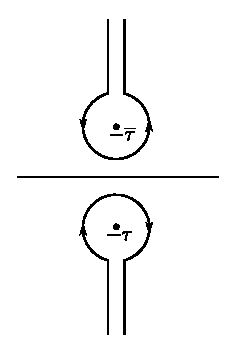
\includegraphics{vol29-fig/fig29-20.eps}
\end{figure}

We decompose $a_n(\tau, s)$ into two parts $b_n(\tau, s)$ and
$c_n(\tau, s)$ such that $a_n(\tau, s)=b_n(\tau, s)+c_n(\tau, s)$ with 
$$
b_n(\tau, s) = \begin{cases}
\oint\limits_{|\tau+u|=\frac{1}{2}y} (\tau+u)^{-2-\frac{s}{2}}
(\overline{\tau}+u)^{-\frac{s}{2}} e^{-2\pi i nu} du \text{ for } n
>0\\
\oint\limits_{|\overline{\tau}+u|=\frac{1}{2}y}
(\tau+u)^{-2-\frac{s}{2}} (\overline{\tau}+u)^{-\frac{s}{2}} e^{-2 \pi
i nu} du \text{ for } n < 0
\end{cases}
$$
and
$$
c_n(\tau, s)=
\begin{cases}
-2 \sin \frac{\pi s}{2} e^{2\pi in\tau}
\int\limits^{\infty}_{\frac{1}{2}y} t^{-2-\frac{s}{2}}
(t+2y)^{-\frac{s}{2}} e^{-2 \pi n t} dt \text{ for } n > 0\\
-2 \sin \frac{\pi s}{2} e^{2\pi i n \overline{\tau}}
\int\limits^{\infty}_{\frac{1}{2}y} (t+2y)^{-2-\frac{s}{2}}
t^{-\frac{s}{2}} e^{2\pi n t} dt \text{ for } n < 0.
\end{cases}
$$

In \pageoriginale any case, $b_n(\tau, s)$ and $c_n(\tau, s)$ are
entire functions of $s$. Moreover, given a compact set $K$ in the
$s$-plane, there exists a positive constant $C=C(y,K)$ such that 
$$
|b_n (\tau,s)|< C e^{-\pi |n|y}, |c_n(\tau, s)| < C e^{-2\pi |n|y}
$$
for $s\in K$ and therefore 
$$
|a_n (\tau, s)| < 2 C e^{-\pi|n|y}
$$

This shows that, if $|Re s |< \sigma_0$ for $s\in K$, then 
$$
4C \sum_{n \neq 0} \left\{ \sum_{\substack{m|n\\m>0}}
m^{\sigma_0-1}\right\}e^{-\pi |n|y}
$$
is a convergent majorant for 
$$
G_2(\tau,s) -2 \zeta(2+s) - 2\zeta(1+s) a_0(\tau,s).
$$
Hence $G_2(\tau,s)-2\zeta(2+s)-2\zeta(1+s)a_0(\tau,s)$ is an entire
function of $s$ and therefore $G_2(\tau, s)$ is regular in the
half-plane $Re s >-1$, in view of our having already proved that
$2\zeta(l+s)a_0(\tau, s)$ is regular for $Re s>-1 $. It follows
immediately from the integral representation of $c_n(\tau,s),
b_n(\tau,s)$ that 
$$
c_n(\tau, 0)=0 \text{ for every } n \neq 0, b_n (\tau,0) = 0 \text{
  for }n < 0
$$
and 
\begin{align*}
b_n(\tau, 0) & = - 2\pi i \text{ res}_{u=-\tau} 
(u+\tau)^{-2} e^{-2\pi i nu}\\
& = -4\pi^2 n e^{2\pi i n \tau} \text{ for } n > 0.
\end{align*}

Substituting \pageoriginale the values of $a_n(\tau,0)$ in (3), we
obtain that
\begin{align*}
G_2 (\tau) = G_2 (\tau, 0) & = 2\zeta(2) - \frac{\pi}{y} - 8\pi^2
\sum^{\infty}_{n=1} \left(\sum_{m n,m>0} m\right) e^{2\pi i n \tau}\\
& = \frac{-2\pi i }{\tau -\overline{\tau}} + \frac{\tau^2}{3} \left\{
1-24 \sum^{\infty}_{n=1} \frac{nq^n}{1-q^n}\right\},
\end{align*}
where $q=e^{2\pi i \tau}$, because
$$ 
\sum^{\infty}_{n=1} \left(\sum_{\substack{m|n\\m>0}} m \right)q^n  =
\sum^{\infty}_{m=1} \sum^{\infty}_{r=1} m q^{mr} = \sum^{\infty}_{m=1}
\frac{mq^m}{1-q^m}. 
$$

Consider the analytic function 
$$
f(\tau) = G_2(\tau) + \frac{2\pi i}{\tau-\overline{\tau}}
=\frac{\pi^2}{3} \left(1-24 \sum^{\infty}_{n=1}
\frac{nq^n}{1-q^n}\right). 
$$

For $S=\left(\begin{smallmatrix} a&b\\c&d \end{smallmatrix}\right)$
in $\Gamma$, it satisfies the transformation formula
$$
f(S<\tau>)(c\tau+d)^{-2} = f(\tau) -\frac{2\pi i c}{c\tau+d},
$$
because $G_2(S<\tau>)(c\tau+d)^{-2}=G_2(\tau)$ and 
$$
\frac{2\pi i}{S<\tau>-S<\overline{\tau}>} (c\tau+d)^{-2} -\frac{2\pi i
}{\tau-\overline{\tau}} = \frac{2\pi i}{\tau-\overline{\tau}}
\left(\frac{c\overline{\tau}+d}{c\tau+d}-1\right) = \frac{-2\pi i c}{c\tau+d}.
$$

In the following, we take for $\log z$ the principal branch i.e. with
$\log z$ real for positive real values of $z$. Let us set 
$$
g(\tau) = 2\pi i \tau + 24 \sum^{\infty}_{n=1} \log(1-q^n).
$$
Then $g'(\tau)=\dfrac{-6}{\pi i}f(\tau)$ and the transformation
formula for $f(\tau)$ implies that \pageoriginale
\begin{align*}
dg(S<\tau>) & = dg(\tau) + \frac{12c}{c\tau+d}d\tau\\
& = dg(\tau) + 12 d(\log(c\tau+d)),
\end{align*}
and therefore
$$
g(S<\tau>) -g(\tau) -12 \log(c\tau+d) = C(S),
$$
where $C(S)$ is a constant depending on $S$. This shows that 
$$
h(\tau) = e^{g(\tau)} = q\prod^{\infty}_{n=1} (1-q^n)^{24}
$$
satisfies the transformation formula

$h(S<\tau>)(c\tau+d)^{-12} = \mathscr{C}(S)h(\tau)$ with
$\mathscr{C}(S)=e^{C(S)}$. By iteration, $\mathscr{C}(S_1 S_2)=
\mathscr{C}(S_1) \mathscr{C}(S_2)$ and
$\mathscr{C}(S)=\mathscr{C}(-S)$. But $h(\tau+1)=h(\tau)$ and
$h(i)\neq 0$; therefore $\mathscr{C}(U)=\mathscr{C}(T)=1$ showing that
$\mathscr{C}(S)=1$ for every $S$ in $\Gamma$. Thus $h(\tau)$ is a
modular form of weight 12 for $\Gamma$, which vanishes at the
parabolic cusp. Hence it follows that $h(\tau)=c\Delta(\tau)$ with
some constant $c$. But the coefficient of $e^{2\pi i \tau}$ in the
Fourier expansion of $h(\tau)$ at $\infty$ is 1, therefore $c=1$ and
we obtain that 
$$
\Delta(\tau) = e^{2\pi i \tau} \prod^{\infty}_{n=1} 
(1-e^{2\pi i n  \tau})^{24}. 
$$
The exact value of the constant $C(S)$ occurring in the transformation
formula for $g(\tau)$ has been computed by Rademacher in \cite{c2:key5}.

\begin{thebibliography}{99}\pageoriginale
\bibitem{c2:key1} R. Fricke and F. Klein: Vorlesungen \"uber die Theorie
  der Elliptischen Modulfunktionen, 2 Bd., Leipzig, 1890.

\bibitem{c2:key2} E. Hecke: Theorie der Eisensteinschen Reihen h\"oherer
  Stufe und ihre Anwendung auf Funktionentheorie und Arithmetik,
  Abh. Math. Sem. Hamburg, 5(1927), 199-224.

\bibitem{c2:key3} A. Hurwitz: \"Uber die Theorie der elliptischen
  Modulfunktionen, Math. Ann., 58 (1904), 343-360.

\bibitem{c2:key4} H. Petersson: \"Uber einen einfachen Typus von
  Untergruppen der Modulgruppe, Archiv der Math., 4 (1953), 308-315.

\bibitem{c2:key5} H. Rademacher: Zur Theorie der Modulfunktionen,
  J. f\"ur reine und angew. Math., 167 (1931), 312-336.

\bibitem{c2:key6} E.C. Titchmarsh: The Theory of the Riemann
  Zeta-Function, Oxford, 1951.

\bibitem{c2:key7} K. Wohlfahrt: \"Uber Dedekindsche Summne und
  Untergruppen der Modulgruppe,  Abh. Math. Sem. Hamburg, 23 (1959),
  5-10. 

\bibitem{c2:key8} K. Wohlfahrt: An extension of F. Klein's level concept,
  Illinois J. of Math., 8 (1964), 529-535.
\end{thebibliography}
